
\documentclass[12pt,a4paper,oneside]{report}
\def\dedication{
  \newpage
  \thispagestyle{empty}    % No page number
  \setcounter{page}{0}
  % \addtocounter{page}{-1}
  \chapter*{}            % Required for \vfill to work
  \thispagestyle{empty}    % No page number
  \null\vfill
  \begin{center}}
\def\enddedication{\end{center}\par\vfill\newpage}

\def\abstract{
  \chapter*{Abstract}
  \addcontentsline{toc}{chapter}{Abstract}
  \relax\markboth{ABSTRACT}{ABSTRACT}}
\def\endabstract{\par\newpage}

\def\abbreviations{
  \chapter*{Abbreviations}
  \addcontentsline{toc}{chapter}{Abbreviations}
  \relax\markboth{ABBREVIATIONS}{ABBREVIATIONS}}
\def\endabstract{\par\newpage}


\def\listoffigure{
  \chapter*{List of Figures}
  \addcontentsline{toc}{chapter}{List of Figures}
\listoffigures
  \relax\markboth{List of Figures}{List of Figures}}
\def\listoffigure{\par\newpage}


\setlength{\textheight}{245mm}
\setlength{\textwidth}{160mm}

\setlength{\headheight}{6mm}
\setlength{\headsep}{12mm}
\setlength{\topmargin}{15mm}

\expandafter\def\expandafter\normalsize\expandafter{%
    \normalsize
    \setlength\abovedisplayskip{15pt}
    \setlength\belowdisplayskip{15pt}
    \setlength\abovedisplayshortskip{15pt}
    \setlength\belowdisplayshortskip{15pt}
}

\usepackage{amsmath}
\usepackage{amsthm}
\usepackage{amssymb}
\usepackage{amsmath}
\usepackage{graphicx}
\usepackage{subfigure}
\usepackage{float}
% \usepackage{epstopdf}
\usepackage{tikz}
%\usepackage{hyperref}

\usepackage{caption}
\usepackage[colorlinks]{hyperref}
\hypersetup{
    colorlinks,%
    citecolor=black,%
    filecolor=black,%
    linkcolor= black,%
    urlcolor=black
}
\usepackage[figure,table]{hypcap}
\usepackage[ruled]{algorithm2e}
\usepackage[top=1in, bottom=1in, left=1in, right=1in]{geometry}
\newcommand{\oneskip}{1.0}
\newcommand{\twoskip}{1.5}
\newcommand{\singlespace}
  {\renewcommand{\baselinestretch}{\oneskip}\Large\normalsize}
\newcommand{\doublespace}
  {\renewcommand{\baselinestretch}{\twoskip}\Large\normalsize}
\usepackage{makeidx}
\usepackage{fancyhdr}
\usepackage[titletoc,page]{appendix}
% \usepackage{bm}
% \usepackage{times}
\usepackage{listings}
\usepackage{color}
\lstset{
    language=C++, 
    breaklines=true, 
    captionpos=b, 
    tabsize=2, 
    frame=single, 
    basicstyle=\footnotesize, 
    showspaces=false, 
    showstringspaces=false, 
    showtabs=true 
}

\usepackage[bottom]{footmisc}


%\newtheorem{theorem}{Theorem}[section]
%\newtheorem{lemma}[theorem]{Lemma}
%\newtheorem{proposition}[theorem]{Proposition}
%\newtheorem{corollary}[theorem]{Corollary}

%=====================================================================
%  Single counter for theorems and theorem-like environments:
%=====================================================================
 \newtheorem{theorem}{Theorem}[chapter]
 \newtheorem{assertion}[theorem]{Assertion}
 \newtheorem{claim}[theorem]{Claim}
 \newtheorem{conjecture}[theorem]{Conjecture}
 \newtheorem{corollary}[theorem]{Corollary}
 \newtheorem{definition}[theorem]{Definition}
 \newtheorem{example}[theorem]{Example}
% \newtheorem{figger}[theorem]{Figure}
 \newtheorem{lemma}[theorem]{Lemma}
 \newtheorem{prop}[theorem]{Proposition}
% \newtheorem{remark}[theorem]{Remark}
\newcommand{\beq}{\begin{equation}}
\newcommand{\eeq}{\end{equation}}
\newcommand{\bea}{\begin{eqnarray}}
\newcommand{\eea}{\end{eqnarray}}

\linespread{2.0}
\makeindex
\begin{document}

\singlespace \begin{titlepage}
    \begin{center}
	%\large{\textbf{Dual Degree Dissertation}} \\
	%\vspace{0.25in}
	\textbf{%
	\vspace{0.05in}
	\Large{\textsc{Sojourn Time of Moving Relays in Dual-Hop Cooperative Communication}}\\ \vspace{0.1in}
	}
	\vspace{0.5in}
	\large Submitted in partial fulfillment of\\
	the requirements for the degree of\\
	\vspace{0.3in}
	\textbf{Bachelor of Technology} \\ \emph{in Electrical Engineering} \\ \& \\ \textbf{Master of Technology} \\ \emph{in Communications and Signal Processing}\\ \vspace{0.05in}

%  (under the Dual Degree Programme) \\
	\vspace{0.30in}
	\large{by}\\
	\vspace{0.30in}

	\large{\textsc{\textbf{Prudhvi Porandla}}}\\110070039

	\vspace{0.6in}
        \normalsize{Under the guidance of}\\ \vspace{0.1in}
% 	\vspace{0in}
	\textbf{\large{	Prof. S. N. Merchant
}}\\
	\vspace{0.2in}

	\begin{figure*}[h]
	\begin{center}
	
\includegraphics[width=1.8in]{images/logo.jpg}
	\end{center}
	\end{figure*}

% 	\vspace{0.1in}
	
	\vspace{-0.2in}
	\large{%
	Department of Electrical Engineering\\
 	\vspace{0.05in}
	Indian Institute of Technology Bombay\\
% 	\vspace{-0.05in}
% 	Powai, Mumbai -- 400076}\\
	% \vspace{0.2in}
	% \date{March, 2007}
	2016
	}

	\end{center}
\end{titlepage}
 \doublespace
\pagebreak
\clearpage\pagenumbering{roman}

 % This makes the page numbers Roman (i, ii, etc)

%\newpage
%\thispagestyle{empty}
%\mbox{}
% %--------------------------------------------------------------------%
% % APPROVAL SHEET
% %   - for final thesis, you need Approval Sheet. So, uncomment the
% %     \makeapproval command.
% %     it should come after dedication, if dedication is
% %     present. Otherwise it is the first page after title page.
% \makeapproval
% \thispagestyle{empty}
% \begin{center}
%   \begin{Huge}
%     \textsc{\textbf{Certificate}}
%   \end{Huge}
% \end{center}
% % \begin{center}
% % Department of Mechanical Engineering\\
% % Indian Institute of Technology Bombay
% % \end{center}
% 
% \vspace{1in}
% \begin{center}
%  Certified that this Dual Degree Project Stage-I Report titled \\ \textit{``\textbf{Next Generation Distributed Cellular Networks} \\ Architecture and Interference Management''} \\by\\Gaurav Varshney (Roll No. 07D07037) \\ is approved by me for submission. \\To the best of my knowledge, the report represents work carried out by the student.\end{center}
% 
% \vspace{1in}
% \begin{table*}[hb]
% \begin{center}
% \begin{tabular}{lr}
% Date: \hspace{1.9in} & \hspace{1.9in} \textbf{Prof. Abhay Karandikar}\\
% \end{tabular}
% \end{center}
% \end{table*}
% \end{certificate}
\newpage

\thispagestyle{empty}
\begin{center}
  \begin{Huge}
    \textsc{\textbf{Dissertation Approval}}
  \end{Huge}
\end{center}

\vspace{0.2in}

 The dissertation entitled \textit{TITLE} by \textit{Prudhvi Porandla (Roll No. 110070039)} is approved for the degree of \textit{Bachelor in Technology} in \textit{Electrical Engineering} and \textit{Master of Technology} in \textit{Communications and Signal Processing.}


\vspace{0.1in}
\begin{flushright}
\textbf{Examiners} \\
\vspace{1.5in}
\textbf{Supervisors}\\
\vspace{1.5in}
 \textbf{Chairman}\\

\end{flushright}
\vspace{0.7in}
Date :    \\
Place :\\
%\begin{table*}[hb]
%\begin{center}
%\begin{tabular}{ll}
%\textbf{Prof.  IITB} & \hspace{0.7in} \textbf{Prof. , IITB}\\
%(Internal Examiner) & \hspace{0.7in} (External Examiner)\\
%\vspace{0.5in}\\
%\textbf{Prof. Rajbabu Velmurugan, IITB} & \hspace{0.7in}  \textbf{Prof. Sibiraj Pillai, IITB} \\ 
%(Guide) & \hspace{0.7in} (Co-Guide)\\
%\vspace{0.5in}\\
%\textbf{Prof. , IITB}\\
%(Chairman)\\
%\end{tabular} \vspace{0.2in}
%\end{center}
%\begin{tabular}{ll}
%Date: & May 22, 2015 \\ \vspace{30pt}
%Place: & Indian Institute of Technology Bombay, Mumbai\\
%\end{tabular}
%
%\end{table*}

%\newpage
%\thispagestyle{empty}
%\mbox{}
%  \newpage
\newpage
\thispagestyle{empty}
\begin{center}
  \begin{Huge}
    \textsc{\textbf{Declaration}}
  \end{Huge}
\end{center}

\vspace{0.5in}

 I declare that this written submission represents my ideas in my own words and wherever others' ideas or words have been included, I have adequately cited and referenced the original sources. I also declare that I have adhered to all principles of academic honesty and integrity and have not misrepresented or fabricated or falsified any idea/ data/ fact/ source in my submission. I understand that any violation of the above will be cause for disciplinary action by IIT Bombay and can also evoke penal action from the sources which have thus not been properly cited or from whom proper permission has not been taken when needed.

\vspace{1.5in}
% \begin{table*}[hb]
% \begin{center}
\hfill \textbf{Prudhvi Porandla}\\
\noindent
\begin{tabular}{ll}
Date: & June 22, 2016\\ \vspace{30pt}
Place: & Indian Institute of Technology Bombay, Mumbai\\
\end{tabular}
% 

% \begin{dedication}
  \newpage
  \thispagestyle{empty}    % No page number

  \begin{center}  \null\vfill
   \textit{\Large To my beloved parents}
  \null\vfill
  \end{center}
% \newpage

% \end{dedication}
%\newpage
%\thispagestyle{empty}
%\mbox{}


\newpage
\thispagestyle{empty}
\begin{center}
  \begin{Huge}
    \textsc{\textbf{Acknowledgements}}
  \end{Huge}
\end{center}

\vspace{0.25in}

I would like to express my sincere gratitude to my supervisor Prof. S. N. Merchant for his invaluable guidance throughout the three years of my association with him. They have always been accessible and willing to clear my doubts and have provided valuable insights that helped me develop new ways to approach the problem and come up with better solutions.\\ %\vspace{0.2in}

\vspace{0.6in}
\noindent June 22, 2016    \hfill \textbf{Prudhvi Porandla}\\


%\newpage
%\thispagestyle{empty}
%\mbox{}


\clearpage\pagenumbering{roman} 
\begin{abstract}

We explore the application of compressed sensing for solving problems in radio astronomy where the source images are generally sparse in some domain. We obtain an incomplete set of noisy Fourier measurements of the image through the radio telescope array and the goal is to reconstruct the image by making use of the sparse nature of the images.

In this report we consider the case where we have multiple sets of Fourier measurements corresponding to different images and in addition we have some knowledge about some overlapping information between the  images. By making use of the overlapping information we should be able to perform better reconstruction than in the case where we perform the reconstruction for the images independently. 

We propose a coupled formulation where we solve a joint minimization problem to perform simultaneous recovery of multiple images. We restrict ourselves to the case where we have two images and present an alternating algorithm that solves the joint minimization problem.

We conduct experiments on different classes of images that include images that are sparse in spatial domain, images that are sparse in wavelet domain and images that are sum of a spatial domain sparse component and a wavelet domain sparse component. In all the cases we observed that the coupled formulation that does simulataneous recovery has better performance as compared to when we perform the reconstructions independently.

 \newpage

\tableofcontents

\listoffigures
  \addcontentsline{toc}{chapter}{List of Figures}
  
\clearpage\pagenumbering{arabic}
\pagestyle{fancy}
\fancyfoot{}                            % Delete current footer settings
%\fancyhf{} %clear all fields
\fancyhead[RO,LE]{\thepage}
\fancyhead[RE]{\leftmark}
\fancyhead[LO]{\rightmark}


\chapter{Introduction}
The broad goal of the field of signal processing is to reconstruct a signal and gain insights into its characteristics based on a series of sampling measurements obtained at discrete time intervals. For a general signal, this task is impossible due to non-availability of data in between two sampling intervals. But, with some prior information about the signal, measurements can be conducted in appropriate ways that enable reconstruction of signals to the desired accuracy.

For example, for a smooth signal which varies slowly with time, sample and hold type of measurements can be conducted to reconstruct the signal to the 
required accuracy.  For another category of signals namely bandlimited signals, the Nyquist-Shannon sampling theorem was an important breakthrough in the field of signal processing. The Nyquist-Shannon sampling theorem states that perfect reconstruction is possible from a set of uniformly spaced samples taken at the Nqyuist rate of twice the highest frequency present in the signal.

Unfortunately, in many applications it may be too costly or physically impossible to build devices capable of sampling at the Nyquist rate or even if it is possible we may end up with far too many samples to efficiently store and process. To address the challenges involved in dealing with such high dimensional data we often depend on compression, which aims to find the most concise representation of a signal that is able to achieve a target level of distortion. Transform coding, one of the most popular techniques for signal compression, relies on finding a basis or a frame that provides sparse or compressible representations for signals in a class of interest. Both sparse and compressible signals can be represented with high fidelity by preserving only the the values and locations of the largest $k$ coefficients of the signals, where $k \ll n$, and $n$ is the length of the signal.

Compressed sensing is a framework for signal acquisition and sensor design that enables a potentially large reduction in the sampling and computation costs for sensing signals that have a sparse or compressible representation. The fundamental idea behind compressed sensing is rather than first sampling at a higher rate and then compressing sampled data, we would like to directly sense the data in compressed form at a much lower sampling rate. The field of compressed sensing grew out of the work of  Candes, Tao and Romberg who showed that, a finite-dimensional signal having a sparse or compressible representation can be recovered from a much smaller number of linear measurements than what Nyquist rate sampling demands \cite{candes,Tao,romberg}. Compressed sensing methods are fast and highly configurable, which makes them highly attractive for a lot of problems such as 
improving MRI imaging \cite{Tao}, developing single pixel cameras \cite{single_pixel}, face recognition algorithms etc. However compressed sensing is still a recent field and its applicability to a large number fields has not yet been fully studied.
Basic information on compressed sensing can be obtained from \cite{cs_rice}. For a complete up-to-date review on compressed sensing refer to \cite{cs_book}. As a part of this thesis, we study the application of compressed sensing methods for improving radio astronomy imaging techniques.

\section*{Compressed Sensing and Radio Astronomy}
Radio Astronomy studies celestial objects at radio frequencies around the metre wavelength, by utilizing the techniques of radio interferometry and aperture synthesis. Mathematically, the problem is equivalent to reconstructing the image of the astronomical object from incomplete and noisy Fourier measurements of the image. From the theory of compressed sensing we know that such measurements may actually suffice for accurate reconstruction of the image provided that the image is sparse in some domain.

Our earlier work \cite{stage1} focused on applying compressed sensing techniques to recover an image of astronomical sources from a an incomplete set of its Fourier measurements. Also, we analyzed the optimality of the GMRT telescope \cite{GMRT} with respect to reconstruction using compressed sensing techniques and came up with optimal antenna locations for additions to the array. 

In this project we consider the case where we have two sets of Fourier measurements corresponding to two different images but in addition we have knowledge about some overlapping information between the two images. The goal is to use this additional information and perform  simultaneous recovery of both images that performs better than if we reconstruct the images independently.  We propose an alternating algorithm that performs simultaneous recovery by solving a joint minimization problem and then conduct experiments to compare the results of the alternating algorithm with those obtained from independent reconstructions. 



\section*{Organization of the report}
The organization of the report is as follows:
\begin{enumerate}

	\item \textbf{Chapter 2} introduces radio astronomy and the basics of radio imaging techniques such as radio interferometry and aperture synthesis.

	\item \textbf{Chapter 3} presents the mathematical model for the compressed sensing problem in a simultaneous recovery setting. We present an alternating algorithm to solve the joint minimization problem to perform simultaneous recovery.

	\item \textbf{Chapter 4} Absorbing MC

	\item \textbf{Chapter 5} analyzes the experiments conducted on simulated data. In this chapter the performance of the alternating algorithm that performs simultaneous recovery is compared against that of the algorithm that reconstructs images separately.

	\item \textbf{Conclusion and Further Work}

\end{enumerate}



%\include{Chapter2_radio_astronomy}
%\include{Chapter3_experiments_results}
%\include{Chapter4_antenna_addition}
%\include{Chapter5_conclusion}
%\include{Chapter2_group_testing}
%\include{Chapter3_adaptive_gt}
%\chapter{Conclusion}
This is where you conclude the report and discuss the significance of your work. Blah blah blah blah blah blah blah blah blah blah blah blah blah blah blah blah blah blah blah blah blah blah blah blah blah blah blah blah blah blah blah blah blah blah blah blah blah blah blah blah blah blah blah blah blah blah blah blah blah blah blah blah blah blah blah blah blah blah blah blah blah blah blah blah blah blah blah blah blah blah blah blah blah blah blah blah blah blah blah blah blah blah blah blah blah blah blah blah blah blah blah blah blah blah blah blah blah blah blah blah blah blah blah blah blah blah blah.
%\include{further_work}


We use stochastic geometry to analyze the performance of a partial decode-and-forward (PDF) relaying scheme applied in a user-assisted relaying setting, where an active user relays data through another idle user in uplink cellular communication. We present the geometric model of a network deploying user-assisted relaying and propose two geometric cooperation policies for fast and slow fading channels. We analytically derive the cooperation probability for both policies. This cooperation
probability is further used in the analytical derivation of the
moments of inter-cell interference power caused by system-wide
deployment of this user-assisted PDF relaying. We then model the
inter-cell interference power statistics using the Gamma distribution by matching the first two moments analytically derived. This
cooperation and interference analysis provides the theoretical
basis for quantitatively evaluating the performance impact of
user-assisted relaying in cellular networks. We then numerically
evaluate the average transmission rate performance and show
that user-assisted relaying can significantly improve per-user
transmission rate despite the increased inter-cell interference. This
transmission rate gain is significant for active users near the
cell edge and further increases with higher idle user density,
supporting user-assisted relaying as a viable solution to crowded
population areas.

\section{Introduction}

\subsection{Motivation}
Mobile subscribers operators and continual driven customer by the increasing demand for number new and
 of
better services place pressing requirements on the underlying
wireless technologies to provide high data rates and wide
coverage. Future generation networks that promise higher data
rates and multifold increase in system capacity include 3GPP
Long Term Evolution-Advanced (LTE-A, 4G) and the emerging 5G systems. The fourth generation (4G) wireless systems were designed to fulfill the requirements of the International Mobile Telecommunications - Advanced (IMT-A). LTE as
a practical 4G wireless system has been recently deployed
in some countries and LTE-A is expected to be deployed
soon around the globe. It is well established that 4G
networks have just reached the theoretical limit on the data
rate with current technologies. These technologies are being
complemented in the fifth generation (5G) wireless systems
by designing and developing new radio concepts to accommodate higher data rates, larger network capacity, higher energy efficiency, and higher mobility necessary to meet the new and challenging requirements of new wireless applications.
5G wireless systems are expected to support peak data rate
of 10 Gb/s for low mobility and 1 Gb/s for high mobility.
These networks are expected to be standardized and deployed around and beyond 2020. Various promising technologies are
proposed for 5G wireless communication systems such as
massive MIMO, energy-efficient communications, Device-to-
Device (D2D) communications, millimeter-wave (mmWave),
and cognitive radio networks.
\par 
D2D and Relaying cooperative communications will play
important roles in future generations wireless networks. D2D
communications enable two proximity users to transmit signal
directly without going through the base station; subsequently,
5G wireless systems are expected to relax the restrictions on
the need to route all user data through the core network. D2D
communications can increase network spectrum utilization and
energy efficiency, reduce transmission delay, offload traffic for
the base station, and alleviate congestion in the cellular core
networks, which make it a promising technology for future
wireless systems. Relay-aided cooperative communi-
cation techniques represent another promising technology that
improves performance in poor coverage areas by enabling
ubiquitous coverage even for users in the most unfavorable
channel conditions. The latest release of the LTE standard
allows the deployment of fixed wireless relays to help cell-
edge mobiles. Yet, other advanced cellular relaying modes are
expected in 5G systems to improve the topology and robustness
of a cellular network and decrease power consumption. These
new technologies include mobile relaying, multi-hop relaying,
and user-equipment based (user-assisted) relaying enabled by
D2D communications 

\subsection{Organization of this report}
This report is in further divided into 6 sections. The topics are organized as follows.
\par Section 2 will discuss partial decode and forward relaying in a standalone setup. The two phases of transmission, signal design and achievable rate of the scheme are presented.
 \par Section 3 is about deployment of the relaying scheme discussed in section 2 in a cellular network. Inter-cell interference and equivalent standard channel model are discussed.
 \par Section 4 contains policies to determine whether the nearest idle neighbour to the active UE can be picked as a relay. Two policies were proposed and analytic expressions for cooperation probabilities were derived.
 \par Section 5 Analytic expressions for interference powers were developed and shape and scale parameters of Gamma distribution that fits interference power statistics were calculated.
 \par Section 6 discusses the simulation setting and how it is different from the theoritical method and the values of parameter used in simulation were listed. It also has simulation results with brief explanations of the result.
 \par Section 7 lists three different topics I'm planning to work on during the second phase. \\
All links/references to equation or figures in this report are clickable.

\pagenumbering{arabic}
\newpage
\section{Partial Decode-and-Forward Relaying}
In this section, we discuss the signal design, channel model and achievable rate of PDF relaying scheme.
\subsection{Signal Design}
Consider a source $\mathcal{S}$, its relay $\mathcal{R}$ and the destination $\mathcal{D}$. Each transmission block is divided into two phases: 1. broadcast transmission in which $\mathcal{S}$ broadcasts to both $\mathcal{R}$ and $\mathcal{D}$. 2. multiple access transmission in which both $\mathcal{S}$ and $\mathcal{R}$ transmit to $\mathcal{D}$. In each block of transmission, $\mathcal{S}$ splits its information into a common part and a private part. The common part is encoded via $U_s^b$ in the 1st phase and $U_s^{m_1}$ in the 2nd phase; and the private part is encoded via $V_s^{m_2}$ in the 2nd phase. The relay $\mathcal{R}$ decodes the information sent by $\mathcal{S}$ in first phase and encodes the same information using $U_s^{m_1}$ in the 2nd phase. \\ 
\begin{figure}[H]
\begin{center}
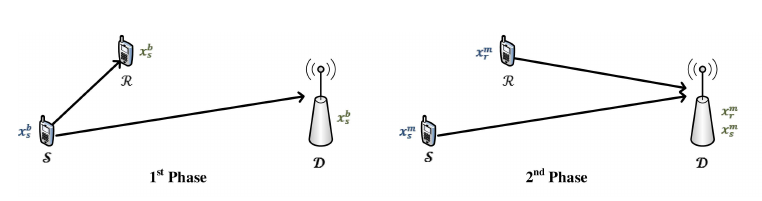
\includegraphics[height = 2in,width=5in,angle=00]{images/pdfRelaying.png}
\caption{\small Transmission phases in PDF relaying}
\label{fig:sysModel}
\end{center}
\end{figure}
The signals transmitted by $\mathcal{R}$ and $\mathcal{S}$ are as follows:
\begin{align}
\text{Phase 1:}\quad x^b_s &= \sqrt{P_s^b} U_s^b, \label{eq:tranSig1}\\
\text{Phase 2:}\quad x_r^m &= \sqrt{P_r^m}U_s^{m_1}, \label{eq:tranSig2}\\ 
 x^m_s &= \sqrt{P_s^{m_1}}U_s^{m_1} + \sqrt{P_s^{m_2}}V_s^{m_2} \label{eq:tranSig3}
\end{align}
All codewords above are picked from independent Gaussian codebooks with zero mean and unit variance. \\ \\
\textbf{Power Constraints:} Let $P_s$ and $P_r$ be the transmit powers of $\mathcal{S}$ and $\mathcal{R}$ respectively and $\alpha_1$ be the fraction of transmission time allocated to first phase, then the following average power constraints should to be satisfied:
\begin{equation}
\alpha_1 P_s^b + \alpha_2 P_s^m = P_s,\quad \alpha_2P_r^m = P_r
\end{equation}
where $\alpha_2 = 1-\alpha_1$

\subsection{Channel Model}
Considering the transmit signals presented above and assuming flat fading over the two phases, the received signals at $\mathcal{R}$ and $\mathcal{D}$ during first phase are 
\begin{equation}
Y_r^b = h_{sr}x^b_s + Z_r^b , \quad Y_d^b = h_{sd}x^b_s + Z_d^b
\end{equation}
where $b$ denotes broadcast mode, $Z_r^b$ and $Z_d^b$ are \textit{i.i.d} circularly-symmetric complex gaussians with mean 0 and variance $\sigma^2$  - $\mathcal{CN}(0,\sigma^2)$ that represent noises at $\mathcal{R}$ and $\mathcal{D}$. \\
Similarly the received signal at $\mathcal{D}$ during second phase can be modelled as 
\begin{equation}
Y_d^m = h_{sd}x^m_s + h_{rd}x_r^m + Z_d^m
\end{equation}
here $m$ denotes multicast transmission; all others have usual meaning.
The above expression is true only if $\mathcal{D}$ has knowledge about the phase offset between $\mathcal{S}$ and $\mathcal{R}$. This assumption is justified by noting that the phase offset between the two nodes can be estimated at base station.

\subsection{Achievable Rate}
With transmit signals in equations~\ref{eq:tranSig1}-~\ref{eq:tranSig3} and joint ML decoding rule at $\mathcal{D}$, the achievable rate for this relaying scheme is:
\begin{equation} \label{eq:rate}
R_{PDF} \leq min(C_1+C_2,C_3)
\end{equation}
\begin{align}
\text{where } C_1 &= \alpha_1 \log\Big(1+|h_{sr}|^2P_s^b\Big),\\
C_2 &= \alpha_2 \log\Big(1+|h_{sd}|^2P_s^{m_2}\Big),\\
C_3 &= \alpha_1 \log\Big(1+|h_{sd}|^2P_s^b\Big) + \alpha_2\log\bigg(1+|h_{sd}|^2P_s^{m_2} + \Big(|h_{sd}|\sqrt{P_s^{m_1}} + |h_{rd}|\sqrt{P_r^m}\Big)^2\bigg)
\end{align}
$C_1$ represents the rate of the common part that can be decoded at $\mathcal{R}$, $C_2$  the private part that can be decoded at $\mathcal{D}$ provided the common part has been decoded correctly, and $C_3$ both the common and private parts that can be jointly decoded at $\mathcal{D}$. These rates are achievable provided full CSI at all receivers and the source-relay phase offset knowledge.
\par
Now that we know what PDF relaying scheme is and the achievable rate, let us see how this scheme performs in cellular networks. To analyse system performance under PDF relaying, we need to know network geometry i.e., how the users and base stations are distributed, how many users can take advantage of relaying, how users identify a potential relay etc. In the next couple of sections we describe network geometry,  received signals and interference model when relaying is deployed in the whole network, and cooperation policies.

\section{Cellular Network Geometry and User-Assisted Relaying}

\subsection{Network geometry model}
Consider a cellular system which consists of multiple
cells, each cell has a single base station and each base station
serves multiple users. Each of the users uses a distinct frequency
block. Each user is served by the single base station that
is closest to that user.


\par We use stochastic geometry to
describe the uplink cellular network. We
assume that the active users in different cells that use the same resource block and cause interference to each other are distributed on a two-dimensional plane according to a homogeneous and stationary Poisson point process (PPP)
$\Phi_1$ with intensity $\lambda_1$. The set of user equipments(UEs) that are in idle state and can participate in relaying are distributed according to another PPP $\Phi_2$ with intensity $\lambda_2$. We assume $\Phi_1$ and $\Phi_2$ are independent. Furthermore, under the assumption that each BS serves a
single mobile in a given resource block, the BS should be closer to its served UE than to any other UE. Therefore we assume each BS is uniformly distributed in the Voronoi cell of its served UE. Fig.~\ref{fig:netLayout} shows an example layout of the network.

\begin{figure}[H]
\begin{center}
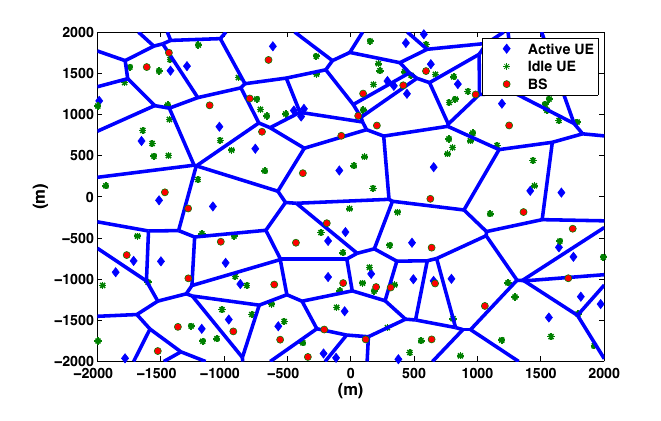
\includegraphics[height = 3in,width=4in,angle=00]{images/netLayoutPaper.png}
\caption{\small Sample layout of a cellular network ($\lambda_2 = 2\lambda_1$)}
\label{fig:netLayout}
\end{center}
\end{figure}

\subsection{Channel Model}
In this section, we describe the channel model when PDF relaying is deployed in cellular network. In this case, there will be out-of-cell inteference in addition to noise. The interference is due to frequency reuse in other cells.
\par Consider $i^{th}$ active UE, we model the received signals at the relay and base station in this cell during 1st phase as
\begin{equation*}
Y_{r,i}^b = h^{(i)}_{sr}x_{s,i}^b + I_{r,i}^b + Z_{r,i}^b,
\end{equation*}
\begin{equation}
Y_{d,i}^b = h^{(i)}_{sd}x_{s,i}^b + I_{d,i}^b + Z_{d,i}^b
\end{equation}
where $I_{r,i}^b$ and $I_{d,i}^b$ represent the interference received at the $i^{th}$ relay and destination. 
\par 
In second phase of the transmission, the received signal at the BS can be modelled as 
\begin{equation}
Y_{d,i}^m = h^{(i)}_{sd}x_{s,i}^m + h^{(i)}_{rd}x_{r,i}^m+ I_{d,i}^m + Z_{d,i}^m
\end{equation}

\subsection{Interference}
To model interference, we assume prefect frame synchronization. LTE-Advanced imposes very strict requirements on synchronization anyway. Interference at the relay during first phase and at the destination(BS) during first and second phases can be expressed as
\begin{equation*} 
I_{r,i}^b = \sum_{k \neq i} B_k h^{(k,i)}_{sr} x_{s,k}^b + (1-B_k)h_{sr}^{(k,i)}x_{s,k} ,
\end{equation*}
\begin{equation*}
I_{d,i}^b = \sum_{k \neq i} B_k h_{sd}^{(k,i)} x^b_{s,k} + (1-B_k)h_{sd}^{(k,i)}x_{s,k},
\end{equation*}
\begin{equation} \label{eq:interferences}
I_{d,i}^m = \sum_{k \neq i} B_k \Big(h_{sd}^{(k,i)} x^m_{s,k} + h_{rd}^{(k,i)} x^m_{r,k}\Big) + (1-B_k)h_{sd}^{(k,i)}x_{s,k}
\end{equation}
the summation is over all active users. Here, $h_{sd}^{(k,i)}$ and $h_{rd}^{(k,i)}$ , respectively, are the channel fading from the $k^{th}$ active UE in $\Phi_1$ and the associated relaying UE in $\Phi_2$ to the BS associated with the $i^{th}$ active UE in $\Phi_1$; and $h_{sr}^{(k,i)}$ is the channel fading from the $k^{th}$ active UE in $\Phi_1$ to the relaying UE associated with the $i^{th}$ active UE in $\Phi_1$.
\par $B_k$ in above expressions is a Bernoulli random variable with success probability $\rho$. $B_k = 1$ is used to indicate the $k^{th}$ active UE's decision to exploit the help of another idle UE, a relay, and apply the relaying transmission strategy, and $B_k = 0$ indicates that the $k^{th}$ UE has no relay. In section~\ref{sec:coop}, we derive the cooperation probability $\rho$ for different cooperation policies.
\par
 For a given setting of nodes locations, based on the
interference model in Eq.~\ref{eq:interferences}, we can use the fact
that interference at either the relay or destination is the
sum of an infinite number of signals undergoing independent fading from nodes distributed in the infinite 2-D plane and use the law of large numbers to approximate the interference as a complex Gaussian distribution.
Also, since the transmitted codewords are complex Gaussian with zero mean, mean of interference is zero. To fully characterize interference as a
complex Gaussian distribution, we define their distributions as $ I_{d,i}^b \sim \mathcal{CN} (0,\mathcal{Q}_{d,i}^b), I_{d,i}
^m \sim \mathcal{CN}(0,\mathcal{Q}_{d,i}^m),$ and $I_{r,i}^b \sim \mathcal{CN}
(0,\mathcal{Q}_{r,i})$ with the variances derived later
in Section~\ref{sec:interference}. The power of these interference terms which
correspond to the variance of the Gaussian random variables
are function of node locations and hence vary with different
network realizations.

\subsection{Equivalent Standard Channel Model}
Using the interference model discussed above, we can convert the channel model in case of relaying into the standard form to capture the effects of
interference into the channel fading as
\begin{align*}
\tilde{Y}_{r,i}^b &= \tilde{h}_{sr}^{(i)}x_{s,i}^b + \tilde{Z}_{r,i}^b, \\
\tilde{Y}_{d,i}^b &= \tilde{h}_{sd}^{(i)}x_{s,i}^b + \tilde{Z}_{d,i}^b, \\
\tilde{Y}_{d,i}^m &= \tilde{h}_{sd}^{(i)}x_{s,i}^m + \tilde{h}_{rd}^{(i)}x_{r,i}^m + \tilde{Z}_{d,i}^m
\end{align*}
where the new channel fading terms are defined as

\begin{equation*}
\tilde{h}_{sr}^{(i)} = \frac{h_{sr}^{(i)}}{\sqrt{\mathcal{Q}_{r,i} + \sigma^2}}, \quad \tilde{h}_{sd}^{(b,i)} = \frac{h_{sd}^{(i)}}{\sqrt{\mathcal{Q}_{d,i}^b + \sigma^2}} \quad
\tilde{h}_{sd}^{(m,i)} = \frac{h_{sd}^{(i)}}{\sqrt{\mathcal{Q}_{d,i}^m + \sigma^2}},
\quad \tilde{h}_{rd}^{(i)} = \frac{h_{rd}^{(i)}}{\sqrt{\mathcal{Q}_{d,i}^m + \sigma^2}}
\end{equation*}
and the noise terms are now all $\mathcal{CN}(0,1)$. Using these equivalent 
standard channels, we can compute the transmission rate using Eq.~\ref{eq:rate}

\section{Cooperation Policies and Probability} \label{sec:coop}
In this section, we look at three cooperation policies: an ideal policy $E_1$, a 
pure geometric policy $E_2$ and a hybrid policy $E_3$ that defines whether an active UE should select an inactive UE to use it in PDF relaying. Also, expressions for cooperation probabilities of $E_2$ and $E_3$ are derived.
\subsection{Policies}
\subsubsection{Ideal Policy $E_1$}
The ideal cooperation policy $E_1$ requires the active UE nodes to know instantaneous  SINRs of the relay link($\mathcal{S}-\mathcal{R}$) and the
direct link($\mathcal{S}-\mathcal{D}$). The policy is defined as 
\begin{align*}
E_1 &= \Big\{|\tilde{h}_{(sr)}^{(k)}|^2 \geq |\tilde{h}_{(sd)}^{(k)}|^2\Big\} \\
&\backsimeq \Big\{ \frac{g_{sr}r_2^{-\alpha}}{\mathcal{Q}_{r,k}} \geq \frac{g_{sd}r_1^{-\alpha}}{\mathcal{Q}_{d,k}^b} \Big\}
\end{align*}
where $r_1$ and $r_2$ denote the direct distance
between $\mathcal{S}$ and $\mathcal{D}$ and cooperation distance between $\mathcal{S}$ and its closest idle UE, respectively and $\alpha$ is pathloss exponent. This event $E_1$ identifies whether an idle UE will be associated as a relay for the $k^{th}$ UE and participate in transmission. Noise variance $\sigma^2$ is ignored since interference power dominates. 
\par Since interference at relay and destination during first phase is more or less the same and $g_{sr}, g_{sd}$ are identically distributed, we can safely ignore them and propose a policy that depends only on distances.

\subsubsection{Pure Geometric Policy $E_2$}
This policy is defined as
\begin{equation}
E_2 = \{r_2\leq r_1, D \leq r_1 \}
\end{equation}
where $D$ is the distance between $\mathcal{R}$ and $\mathcal{D}$. In words, if source's(active UE's) nearest idle neighbour is in the intersection region of two circles of radius $r_1$ centered at source and destination, then that idle UE will be chosen to act as a relay.
\par $E_2$ is more practical than policy $E_1$ in the sense that
it does not require full knowledge of both the channel fading
and the interference at the decision making node. Instead, it
only requires the decision making nodes to know the distances
from the active user to the nearest idle user and to the base
station. It represents a practical decision making strategy for
fast fading channels, requiring no knowledge of the channel
fading. 
\subsubsection{Hybrid Policy $E_3$}
This policy is proposed for slow fading channels where small scale fading parameters estimation and their
feedback to the decision making node is feasible. 
\begin{equation}
E_3 = \{g_{sd}r_1^{-\alpha} \leq g_{sr}r_2^{-\alpha}, D \leq r_1 \}
\end{equation}
Note that this cooperation policy is still independent of the
interference as in the pure geometric cooperation policy $E_2$.

\subsection{Cooperation Probabilities}
In this part of the section we derive cooperation probabilities $\rho_2$ and $\rho_3$ for the policies $E_2$ and $E_3$ respectively. For the ideal policy $E_1$, analytic evaluation of the
cooperation probability is rather complicated because of the
inter-dependency between the cooperation decision and consequential interference among different cells. Consider a random BS and its associated active UE. 
The distribution of the distance
$r_1$ between the $i^{th}$ UE and its associated BS can be shown to
be Rayleigh distributed directly from the null probability of a
two dimensional PPP distribution. 
\par  Due to the stationarity of the
PPP, i.e., location of the origin doesn't change the distribution of points, and the independence of $\Phi_2$ from BSs distribution we can assume that
the location of the UE associated with the BS under study
represents the origin point of $\Phi_2$ . Then, each UE
in $\Phi_1$ chooses the closest UE in $\Phi_2$ to assist it in relaying
its message to the serving BS. Hence, similar to source-to-
destination distance, the distribution of the source-to-relay
distance $r_2$ between the $i^{th}$ UE and its associated relaying UE
can be also shown to be Rayleigh distributed from the null probability of a two dimensional PPP. Therefore,
\begin{equation*}
f_{r_1}(r_1) = 2\pi\lambda_1r_1e^{-\lambda_1\pi r_1^2},
\end{equation*}
\begin{equation}
f_{r_2}(r_2) = 2\pi\lambda_2r_2e^{-\lambda_2\pi r_2^2}
\end{equation}

\begin{theorem}{Cooperation Probabilities.}
The probability of
deploying user-assisted relaying for a randomly located active
user within a cell can be evaluated as follows:
\begin{itemize}
\item[i.] For policy $E_2$
\begin{equation}
\rho_2 = \int_{-\pi/2}^{-\pi/3}\frac{2\lambda_2 cos^2\psi_0}{\pi(\lambda_1+4\lambda_2cos^2\psi_0)}d\psi_0 + \int_{\pi/3}^{\pi/2}\frac{2\lambda_2 cos^2\psi_0}{\pi(\lambda_1+4\lambda_2cos^2\psi_0)}d\psi_0 + \frac{\lambda_2}{3(\lambda_1+\lambda_2)}
\end{equation}
\item[ii.] For policy $E_3$
\begin{align*}
\rho_3 &= \int_0^2 f_{\beta}(z)\int_{-\pi/2}^{-cos^{-1}(z/2)}\frac{2\lambda_2 cos^2\psi_0}{\pi(\lambda_1+4\lambda_2cos^2\psi_0)}d\psi_0 dz \\ 
&+ \int_0^2 f_{\beta}(z)\int^{\pi/2}_{cos^{-1}(z/2)}\frac{2\lambda_2 cos^2\psi_0}{\pi(\lambda_1+4\lambda_2cos^2\psi_0)}d\psi_0 dz \\ &+\int_0^2 f_{\beta}(z)\frac{\lambda_2 z^2 cos^{-1}(z/2)}{\pi(\lambda_1+\lambda_2z^2)}dz \\ 
&+ \int_2^{\infty} f_{\beta}(z)\int_{-\pi/2}^{\pi/2}\frac{2\lambda_2 cos^2\psi_0}{\pi(\lambda_1+4\lambda_2cos^2\psi_0)}d\psi_0 dz
\end{align*}
where $\beta = \bigg(\frac{g_{sr}}{g_{sd}}\bigg)^{1/\alpha}$ and $f_{\beta}(z)$ is pdf of $\beta$ which can be shown to be 
\begin{equation}
f_{\beta}(z) = \frac{\alpha z^{\alpha-1}}{(1+z^{\alpha})^2}
\end{equation}
\end{itemize}
\end{theorem}
\begin{proof}
\begin{itemize}
\item[i.] 
\begin{align*}
\rho_2 &= \mathbb{P}\{E_2\} \\
&= \mathbb{P}\{r_2 \leq r_1, r_1^2+r_2^2-2r_1r_2cos\psi_0 \leq r_1^2\} \\
&= \mathbb{P}\{r_2 \leq r_1, r_2 \leq 2 r_1 cos\psi_0 \} \\
\end{align*}
when $|\psi_0|<\pi/3, ~ r_1 < 2r_1cos\psi_0  \Rightarrow \text{ if } r_2 < r_1 \text{, $r_2$ satisfies both inequalities.}$ Accordingly, we define $\mathcal{E}_1$ and $\mathcal{E}_2$ as follows
\begin{align*}
\mathcal{E}_1 &= (2\pi)^2\lambda_1 \lambda_2 \int_0^\infty \int_0^{2r_1 cos\psi_0}r_1r_2e^{-\pi(\lambda_1 r_1^2 + \lambda_2 r_2^2)}dr_2 dr_1 \\
&= \frac{2\lambda_2 cos^2\psi_0}{\pi(\lambda_1+4\lambda_2cos^2\psi_0)} \\
\mathcal{E}_2 &= (2\pi)^2\lambda_1 \lambda_2 \int_0^\infty \int_0^{r_1}r_1r_2e^{-\pi(\lambda_1 r_1^2 + \lambda_2 r_2^2)}dr_2 dr_1 \\
&= \frac{\lambda_2}{2\pi(\lambda_1+\lambda_2)}
\end{align*}
 
\begin{align*}
\text{Now, }\rho_2 &= \int_{-\pi/3}^{\pi/3} \mathcal{E}_2 d\psi_0 + 2\int_{\pi/3}^{\pi/2} \mathcal{E}_1d\psi_0 \\
&=  \frac{\lambda_2}{3(\lambda_1+\lambda_2)} + 2\int_{\pi/3}^{\pi/2} \mathcal{E}_1d\psi_0
\end{align*} 

\item[ii.]
\begin{align}
\rho_3 &= \mathbb{P}\{E_3\} \\
&= \mathbb{P}\{r_2 \leq \bigg(\frac{g_{sr}}{g_{sd}} \bigg)^{1/\alpha}r_1, r_1^2+r_2^2-2r_1r_2cos\psi_0 \leq r_1^2\} \\
&= \mathbb{P}\{r_2 \leq \beta r_1, r_2 \leq 2 r_1 cos\psi_0 \} \\
&= \mathbb{P}\{r_2 \leq 2 r_1 cos\psi_0 \} \qquad \text{ for } \beta > 2 \\
&= \mathbb{P}\{r_2 \leq \beta r_1\} \qquad \text{ for } \beta < 2  \text{ and } |\psi_0| < cos^{-1}(\beta/2) \\
&= \mathbb{P}\{r_2 \leq 2 r_1 cos\psi_0 \} \qquad \text{ for } \beta < 2 \text{ and } cos^{-1}(\beta/2) < |\psi_0| <  \pi/2 \\
\therefore \rho_3&= 2 \int_0^2 f_{\beta}(z)\int^{\pi/2}_{cos^{-1}(z/2)}\mathcal{E}_1 d\psi_0 dz +\int_0^2 f_{\beta}(z)\int_{-cos^{-1}(z/2)}^{cos^{-1}(z/2)}\mathcal{E}_3 d\psi_0dz \\&+ \int_2^{\infty} f_{\beta}(z)\int_{-\pi/2}^{\pi/2}\mathcal{E}_1 d\psi_0 dz \label{eq:corrected}
\end{align}

$\mathcal{E}_1$ is defined in part i. of the proof and  $\mathcal{E}_3 = \frac{\lambda_2 z^2}{2\pi(\lambda_1+\lambda_2z^2)}$ which is nothing but $\mathcal{E}_2$ with $\lambda_2 = \lambda_2z^2$. $f_\beta(z)$, the pdf of $\beta$, can be obtained as follows

\begin{align*}
F_\beta(z) &= \mathbb{P}\bigg\{ \bigg( \frac{x_1}{x_2}\bigg)^{1/\alpha} \leq z \bigg\} = \mathbb{P} \{ x_1\leq z^\alpha x_2\} \\
&= \int_0^\infty \int_0^{z^\alpha x_2} e^{-(x_1+x_2)} dx_1dx_2 \quad \text{ since } g_{sr},g_{sd} \sim Exp(1) \\
&= 1-\frac{1}{1+z^\alpha}, \qquad z \in [0,\infty)
\end{align*}
The pdf $f_\beta(z)$ is then obtained by differentiating $F_\beta(z)$ :
\begin{equation*}
    f_\beta(z) = \frac{dF_\beta(z)}{dz} = \frac{\alpha z^{\alpha-1}}{(1+z^\alpha)^2} \quad z \in [0,\infty)
\end{equation*}
\end{itemize}
\end{proof}
\section{Interference Analysis} \label{sec:interference}
User-assisted relaying actually increases the amount of out-
of-cell interference in the network as some idle users are now
transmitting when relaying information of active users. It is
therefore necessary to understand this out-of-cell interference
power, particularly its distribution, in order to assess the overall
impact of user-assisted relaying on system performance.
\subsection{First Two Moments of Interference Power} Since it is difficult to describe the
exact distribution of out-of-cell interference power, here we
choose to model the interference power to the cell under study
as a Gamma distribution by fitting the first two moments of
the interference power analytically developed using stochastic
geometry of the field of interferers outside that cell.
The expressions for interference power can be developed from Eqs.~\ref{eq:interferences}. 
\begin{align}
\mathcal{Q}_{d,i}^b &= \sum_{k\neq i}B_k \Big |h_{sd}^{(k,i)}\Big|^2P_{s,k}^b + (1-B_k)\Big|h_{sd}^{(k,i)}\Big|^2P_{s,k} \\
\mathcal{Q}_{d,i}^m &= \sum_{k\neq i}\bigg[B_k\bigg(\Big|h_{sd}^{(k,i)}\Big|^2 P_{s,k}^m+\Big|h_{rd}^{(k,i)}\Big|^2 P_{r,k}^m\bigg)\bigg] + (1-B_k) \Big| h_{sd}^{(k,i)}\Big|^2 P_{s,k} \\
\mathcal{Q}_{r,i} &= \sum_{k\neq i}B_k \Big|h_{sr}^{(k,i)}\Big|^2P_{s,k}^b + (1-B_k)\Big|h_{sr}^{(k,i)}\Big|^2P_{s,k} 
\end{align}
\begin{theorem}{Interference Power Statistics} \label{theorem:theorem2}
For network-wide
deployment of user-assisted relaying, the out-of-cell interfer-
ence generated at the destination BS and the relaying UE have
the following statistics:

\begin{itemize}
\item[i.] 
The first two moments, mean and variance, of interference
power at the destination BS during the 1st and 2nd phase,
respectively, are
\begin{equation}
\mathbb{E}[\mathcal{Q}_{d,i}^b] = \frac{2\pi\lambda_1\zeta_1}{\alpha-2}R_c^{2-\alpha}, \qquad \mathbb{E}[\mathcal{Q}_{d,i}^m] = \frac{2\pi\lambda_1\zeta_3}{\alpha-2}R_c^{2-\alpha}
\end{equation}
\begin{equation}
\text{var}[\mathcal{Q}_{d,i}^b] = \frac{\pi\lambda_1\zeta_2}{\alpha-1}R_c^{2(1-\alpha)}, \qquad \text{var}[\mathcal{Q}_{d,i}^m] = \frac{\pi\lambda_1\zeta_4}{\alpha-1}R_c^{2(1-\alpha)}
\end{equation}

\item[ii.]
The first two moments, mean and variance, of interfer-
ence power at the idle UE associated as a relay with the ith
active UE are
\begin{equation}
\mathbb{E}[\mathcal{Q}_{r,i}] = \lambda_1\zeta_1 \int_0^{2\pi}\int_{R_c}^\infty (r^2+D^2-2rDcos\theta)^{\alpha/2}rdrd\theta
\end{equation}
\begin{equation}
\text{var}[\mathcal{Q}_{r,i}] = \lambda_1\zeta_2 \int_0^{2\pi}\int_{R_c}^\infty (r^2+D^2-2rDcos\theta)^{\alpha/2}rdrd\theta
\end{equation}

\begin{align} \label{eq:zeta1}
\text{where} \quad  \zeta_1 &= \rho_1 P_{s,k}^b +(1-\rho_1)P_{s,k} \\
                \zeta_2 &= 2[\rho_1(P_{s,k}^b)^2 + (1-\rho_1)P_{s,k}^2],\\
                \zeta_3 &= \rho_1 (P_{s,k}^m+P_{r,k}^m) +(1-\rho_1)P_{s,k}, \\
                \zeta_4 &= 2[\rho_1(P_{s,k}^m+P_{r,k}^m)^2 + (1-\rho_1)P_{s,k}^2 -\rho_1P_{s,k}^mP_{r,k}^m] \label{eq:zeta4}
\end{align}
\end{itemize}
\end{theorem}
\begin{proof}
\begin{align*}
\mathbb{E}[\mathcal{Q}_{d,i}^b] &= -\frac{\partial\mathcal{L}_{\mathcal{Q}_{d,i}^b}(s)}{\partial s}\bigg\rvert_{s=0}, \\
\text{var}[\mathcal{Q}_{d,i}^b] &= -\frac{\partial^2\mathcal{L}_{\mathcal{Q}_{d,i}^b}(s)}{\partial s^2}\bigg\rvert_{s=0} - \Big(\mathbb{E}\big[\mathcal{Q}_{d,i}^b \big] \Big)^2
\end{align*}
where $\mathcal{L}_{\mathcal{Q}_{d,i}^b}(s)$ is the Laplace transform of $\mathcal{Q}_{d,i}^b$ and $R_c = 1/2\sqrt{\lambda_1}$ is the cell radius. Means and variances of $\mathcal{Q}_{d,i}^m$, $\mathcal{Q}_{r,i}$ can be calculated similarly.
\end{proof}
\par From the above results for interference power statistics, the interference power is directly proportional to both
the active users density, $\lambda_1$ , and the transmission power levels
represented by $\zeta_i , i \in [1:4] $ in Eqs.~\ref{eq:zeta1} - ~\ref{eq:zeta4}

\subsection{Modelling Interference Power Distribution}
A parameterized probability distribution, which includes a
wide variety of curve shapes, is useful in the representation of
data when the underlying model is unknown or difficult to obtain in closed form. A parameterized probability distribution is
usually characterized by its flexibility, generality, and simplicity. Although distributions are not necessarily determined by
their moments, the moments often provide useful information
and are widely used in practice. It is shown that the Gamma
distribution is a good approximation for the interference when
the point under study is closer to the cell center, but fails
to represent the actual interference distribution whenever the
point under study is exactly at the cell edge. We use the same
approach here and match a Gamma distribution to the first
two moments of the interference power terms derived earlier
in Theorem~\ref{theorem:theorem2}.
\subsubsection{Gamma Distribution}
The Gamma distribution is specified by a shape parameter $k$ and a scale parameter $\theta$. The pdf of a Gamma distributed RV $\gamma[k,\theta]$ is defined as 
\begin{equation*}
F_\gamma(q|k,\theta) = \frac{q^{k-1}e^{(-q/\theta)}}{\theta^k\Gamma(k)}
\end{equation*}
where the Gamma function $\Gamma(t)$ is defined as $\Gamma(t) = \int_0^{\infty}x^{t-1}e^{-x}dx$. The mean and variance of $\gamma[k,\theta]$ are $k\theta$ and $k\theta^2$ respectively.
\par
Since we know mean and variance of interference powers, we can estimate the shape and scale parameters by using the formulae:
\begin{equation}
k_i = \frac{(\mathbb{E}[\mathcal{Q}_i])^2}{\text{var}[\mathcal{Q}_i]}, \theta_i =\frac{\text{var}[\mathcal{Q}_i]}{\mathbb{E}[\mathcal{Q}_i]}
\end{equation}

\section{Simulations and Results}

\subsection{Simulation Setting}

All simulations were done on a square region of side length 200m. 
To generate active UEs in the region, the number of UEs is taken as a realization of poisson RV with parameter $\lambda_1$ and these number of UEs were uniformly distributed in the square region. The same is done to generate idle UEs but with parameter $\lambda_2$. I discarded the UEs whose Voronoi region extends to infinity. 
\par In theory, the base station of a UE is uniformly distributed in the Voronoi region of UE but there is no easy practical way to uniformly pick a point from a polygonal area. One method is to triangulate the polygonal Voronoi region, choose a triangle weighted by area, choose a point inthat triangle. This is clearly quite complex to code so I've not implemented this method. The method I followed to generate BSs is - pick a number greater than or equal to the number of active UEs and distribute these number of BSs uniformly in the square region. Now go to each active UE and check if there are any BSs in its Voronoi region. If there are BSs, pick one of them and associate it with the UE and discard other BSs in the Voronoi region. Since BSs are distributed uniformly over the whole region, the result is as good as picking BSs uniformly in the Voronoi regions of UEs which is what we wanted but there is a catch. In the theoritical method, each UE with a finite Voronoi region is guaranteed to have a BS whereas in the way that I'm generating, some UEs might not have a BS even though their Voronoi region is of finite area. Further, the UEs without a BS are not included in rate or cooperation probability analysis which is logical since without an associated BS, the UEs cannot considered active.
\par For all simulations, we assume that UEs are using maximum power to transmit without applying any power control method.\label{sec:powerCon}  The powers used during the two phases of transmission are as follows
\begin{itemize}
\item Source and relays use equal power $\Rightarrow P_{s,i} = P_{r,i} $ 
\item Source use equal power during broadcast and multicast phases $\Rightarrow P_{s,i}^b = P_{s,i}^m$ 
\item $P_{s,i}^{m_1} = \beta_1 P_{s,i}^m$ and $P_{s,i}^{m_2} = (1-\beta_1) P_{s,i}^m$. Where $\beta_1$ is allocated optimally to maximize the transmission rate of the active user. To do this, rate is expressed as a function of $\beta_1$ and minimized negative rate using MATLAB tool \textit{fminrnd}.
\end{itemize}
\subsection{Results}
\begin{figure}[H]
\begin{center}
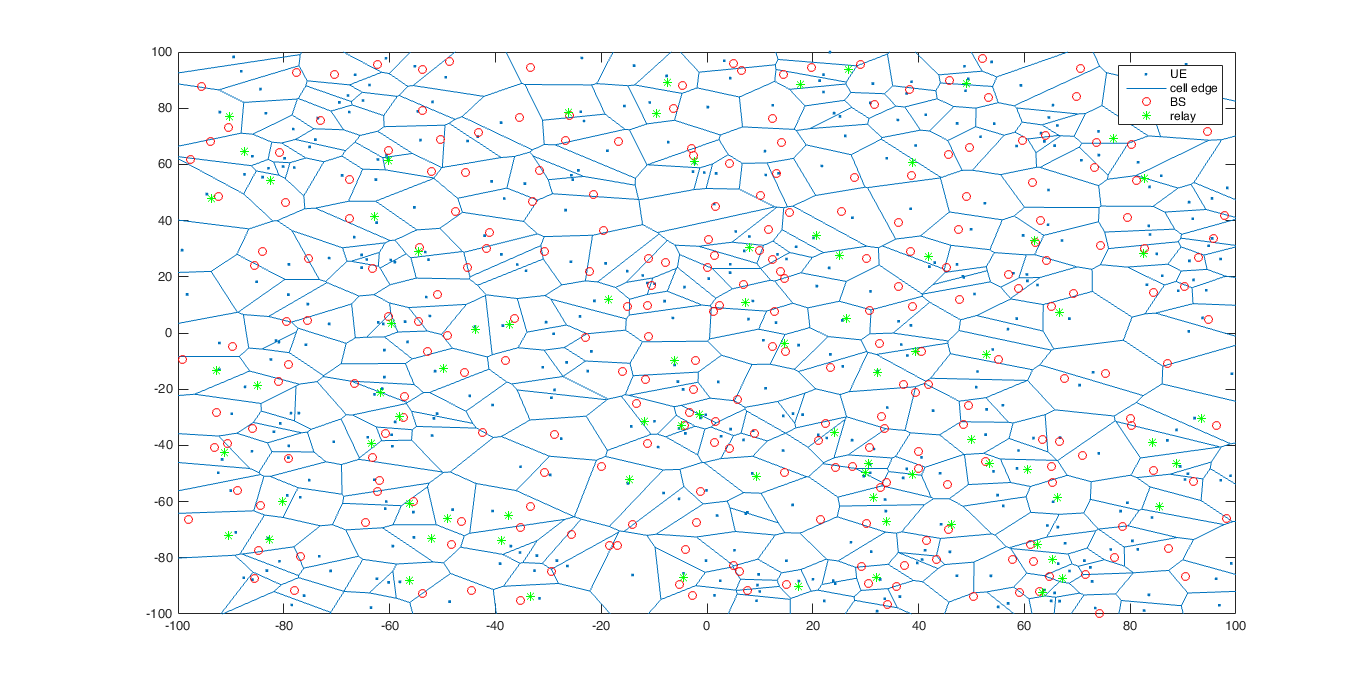
\includegraphics[height = 4in,width=7in,angle=00]{images/netLayoutSim.png}
\caption{\small Network Layout}
\label{fig:netLayoutSim}
\end{center}
\end{figure}
This a sample network layout generated by using the method discussed in previous subsection. We can see that some of the UEs are well within the range but have no BS. Only UEs with a BS are considered active. A fraction active UEs have relays, these UEs use PDF relaying. Cooperation probability = number of active UEs with relays/total number of active UEs.
\begin{figure}[H]
\begin{center}
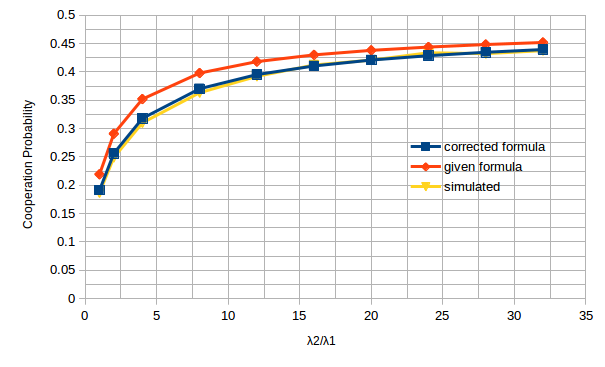
\includegraphics[height = 3in,width=4in,angle=00]{images/corrected.png}
\caption{\small Corrected cooperation probability of $E_3$}
\label{fig:correctedE3}
\end{center}
\end{figure}
In the published paper, the analytic result for cooperation probability of $E_3$ has an error. The correction being using $\mathcal{E}_3$ instead of $\mathcal{E}_2$ in eq.~\ref{eq:corrected}. The corrected analytic result matches the simulation result as can be seen in the above figure. 
\begin{figure}[H]
\begin{center}
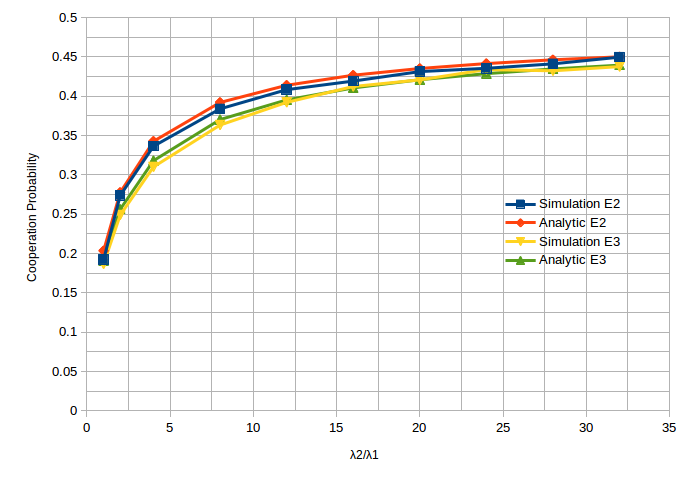
\includegraphics[height = 3in,width=4in,angle=00]{images/coopP.png}
\caption{\small Cooperation probabilities of $E_2$, $E_3$ versus user density ratio}
\label{fig:cooP}
\end{center}
\end{figure}
From the above graph we can see that cooperation probability of both policies increases with user density ratio($\lambda_2/\lambda_1$) and reach a maximum of 0.5 for very large user density ratio. Also, the analytic and simulations results closely match. 

\begin{figure}[H]
\begin{center}
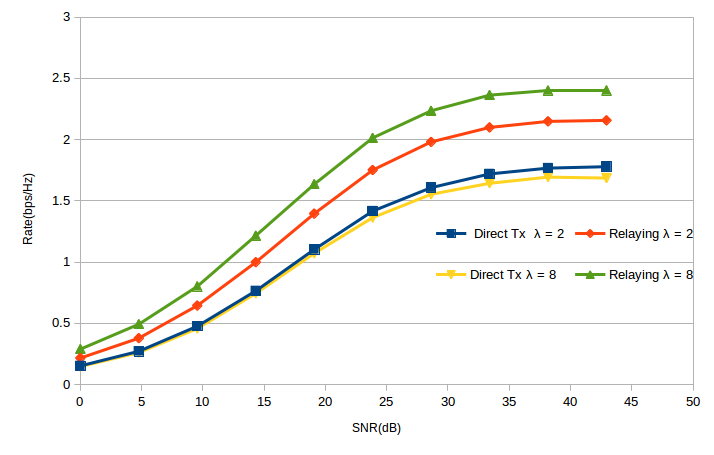
\includegraphics[height = 2.8in,width=4in,angle=00]{images/rates.png}
\caption{\small Average rate per user; $\lambda = \lambda_2/\lambda_1$}
\label{fig:rates}
\end{center}
\end{figure}
From the above figure, we can clearly see that average rate per user has increased when PDF relaying is deployed over the whole network. The rate also increases as user density ratio is increased but we caan't sure whether the rate keeps increasing with $\lambda$. It might happen that the rate decreases for very large user ratio density due to increase in interference.

\chapter{Joint reconstruction from multiple observations}
In the previous chapter we saw that the problem is to determine the image(i.e intensity distribution) from an incomplete set of Fourier measurements since we have data available only at certain points in the Fourier domain, determined by the $u-v$ coverage of the antenna setup. In general we assume that we have data available at points in the Fourier domain determined by the ``sampling map''.  Next we present the problem formulation.
\section{Problem Formulation}
We consider the problem where we have two incomplete sets of Fourier measurements corresponding to two different images and further we have knowledge about some information overlap between the two images. We want to make use of this overlapping information to perform simultaneous recovery of both images.  Next we formulate the simultaneous recovery problem,

 Let $x$ and $y$ be the discretized vectors of the lexicographic ordering of the intensity distributions (i.e. the images) of size $N \times 1$.
 Corresponding to each image we have a set of linear measurements obtained as,
 \begin{eqnarray}
  b_x &=& \Phi_x x  + n_x\\
  b_y   &=& \Phi_y y + n_y,
 \end{eqnarray}
where $\Phi_x$ and $\Phi_y$ are $M_x \times N$ and $M_y \times N$ measurement matrices respectively and $n_x$ and $n_y$ are terms corresponding to the noise added to the system while obtaining the measurements ($M_x < N, \ M_y < N)$. 

Let both $x$ and $y$ be sparse/compressible in the same basis and thus they can be represented as,
\begin{eqnarray}
	x &=& \Psi z_x 	\label{eq:domainx}\\
	y &=& \Psi z_y,
	\label{eq:domainy}
\end{eqnarray}
where $z_x$ and $z_y$ are $N \times 1$ sized vectors containing only few non-zero/large coefficients and $\Psi$ is the  $N \times N$  matrix with columns as the basis vectors of the desired basis. 

Let there be some information overlap between $x$ and $y$. We will restrict ourselves to only those features that can be extracted through a linear operation on the images. Let $f_x$ and $f_y$ be the $S \times 1$ feature vectors obtained from $x$ and $y$ as,
\begin{eqnarray}
f_x &=& B_x z_x\\
f_y &=& B_y z_y,
\end{eqnarray}
where $B_x$ and $B_y$ are $S \times N$ feature extraction matrices. For example if the last $c$ columns of image corresponding to $x$ overlap with the first $c$ columns of the image corresponding to $y$ then $B_x$ and $B_y$ will be $cn \times N$ matrices where we assume the images to be of size $n \times n$ and $N = n^2$. $B_x$ and $B_y$ will have rows with all entries zero except the position corresponding to the location of a certain pixel in the lexicographic ordering of the image. Under ideal reconstruction, the two feature vectors must match because they correspond to the overlapping part.
\begin{equation}
||f_x - f_y||_2^2 < \epsilon_f,
\end{equation}
where $\epsilon_f$ is some tolerance threshold. 
Next we present several formulations that can be used to solve this problem:
\begin{enumerate}
\item \textbf{Formulation-1} 
Using conventional compressed sensing methods, we will first solve for $z_x^*$ and $z_y^*$ independently  as follows and obtain $x^*$ and $y^*$ using (\ref{eq:domainx}) and  (\ref{eq:domainy}):
\begin{eqnarray}
 z_x^* &=&  \arg \min_{z_x} \| z_x \|_1 \ \text{for} \ \|\Phi_x \Psi z_x -b_x\|_2^2 \leq \epsilon_x \\
 z_y^* &=&  \arg \min_{z_y} \| z_y \|_1 \ \text{for} \ \|\Phi_y \Psi z_y -b_y\|_2^2 \leq \epsilon_y,
 \label{form1}
\end{eqnarray}
where $\epsilon_x$ and $\epsilon_y$ are variances corresponding to $n_x$ and $n_y$ respectively.
\item \textbf{Formulation-2} There is an alternative formulation which allows for unconstrained optimization.
\begin{eqnarray}
 z_x^* &=& \arg \min_z F(z) \equiv \|\Phi_x\Psi z - b_x\|_2^2 + \lambda_x \|z\|_1\\
 z_y^* &=& \arg \min_z F(z) \equiv \|\Phi_y\Psi z - b_y\|_2^2 + \lambda_y \|z\|_1,
\label{form2}
 \end{eqnarray}
where $\lambda_x$ and $\lambda_y$ must be chosen appropriately to obtain same results as obtain using \emph{formulation-1}.
Greedy methods such as ISTA and FISTA make use of this formulation to solve the problem.
\item \textbf{Formulation-3} Instead of solving for $x$ and $y$ separately we can solve for them simultaneously making use of the information overlap by the following formulation for unconstrained optimization,
 \begin{equation}
 z_x^*, z_y^* = \arg \min_{z_x, z_y} F(z_x, z_y),
 \end{equation}
where,
 \begin{equation}
 F(z_x, z_y) \equiv \|\Phi_x\Psi z_x - b_x\|_2^2 + \|\Phi_y\Psi z_y - b_y\|_2^2 + \lambda_x \|z_x\|_1 + \lambda_y \|z_y\|_1 + \mu ||f_x - f_y||_2^2.
 \label{eq:formu}
 \end{equation}
Here, we have the four terms present from Formulation-2 but in addition we have a ``\emph{coupling term}''  $||f_x - f_y||_2^2$ along with the ``\emph{coupling parameter}'' $\mu$. The parameter $\mu$ will decide the degree of overlap in the reconstructed images and setting $\mu = 0$ will revert back to Formulation-2.
Here $\lambda_x$, $\lambda_y$ and $\mu$ must be chosen appropriately to ensure convergence to correct results. We propose an alternating algorithm to solve this optimization problem which is in similar lines to the ISTA or FISTA algorithm in one argument.
This formulation reduces to the formulation JSM-1 presented in \cite{JSM} when $B_x = B_y$, but with a subtle difference.  In the formulation presented in \cite{JSM} the common part has to be same at every iteration of the algorithm but in our formulation we allow the common part in both images to take different values during the course of the algorithm but reach close to being same at convergence depending upon the weight $\mu$.

\end{enumerate}
\section{Alternating Algorithm for Simultaneous Recovery}
The alternating algorithm is a generalization of the ISTA  which is a proximal gradient algorithm. We first  briefly look at proximal methods and then the ISTA and FISTA algorithm and finally present the alternating algorithm.
\subsection{Proximal Methods}
Proximal methods are a higher level of abstraction than classical optimization algorithms such as gradient descent. The basic constituent of a proximal method is the \emph{proximal operator}, which essentially solves a simple convex optimization problem \cite{prox_book}. The proximal operator for the scaled function $f$ at a point $x$ with respect to parameter $\lambda$ is given by,
\begin{equation}
prox_{\lambda f}(x) = \arg \min_y \left( f(y) + \frac{1}{2\lambda} \| x - y \|^2. \right)
\end{equation}
We refer to $prox_{\lambda f}(x)$ as the proximal operator of $f$ with respect to parameter $\lambda$ at point $x$.
Here the $\|\| x - y \|\|^2$ term keeps the mapped point in the proximity of the argument $x$ and the $\min f(y)$ term, drives the mapped point towards the minima of the function f. The parameter $\lambda$ decides which of the two factors dominates.


\begin{figure}[h]
	\centering \vspace{-0.1in}
	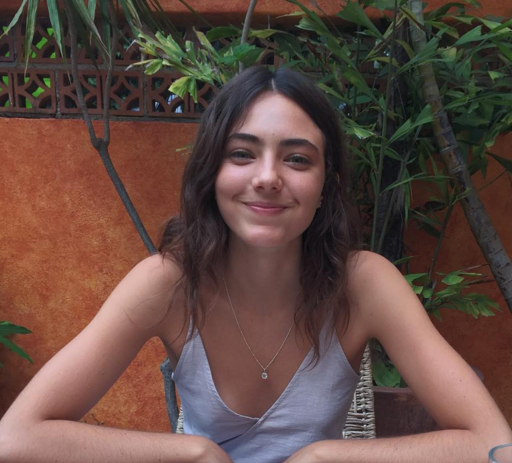
\includegraphics[width=0.6\textwidth]{images/proximal.png}	
	\vspace{-20pt} \caption[Effect of the proximal Operator]{\small Effect of the Proximal Operator \footnotemark}
	\label{fig:proximal_operator}
\end{figure}
\footnotetext{Image Source: \url{http://www.stanford.edu/~boyd/papers/pdf/prox_algs.pdf}}
Consider the figure \ref{fig:proximal_operator}. Here, the proximal operator maps the blue points to the red points.
The mapped points come closer to the minima, but still remain in proximity of the original blue point.

\subsection{Proximal operator for smooth functions}


\begin{enumerate}
\item Consider a smooth function $f(x)$.
\item The proximal operator for $f$ with respect to parameter $t$ at point $x$ is given by:
\begin{equation}
 prox_{tf}(x) = \arg \min_y  \left( f(y) + \frac{1}{2t} \|x-y\|^2  \right).
\end{equation}
As, the mapped point is expected to be in the proximity of the original point $x$, we use a linear approximation of $f(y)$ at $x$  and thus we have,

\begin{equation}
 prox_{tf}(x) = \arg \min_y \left( f(x) + (y-x)^T \nabla f(x)  + \frac{1}{2t} \|x-y\|^2 \right).
\end{equation}
\item On simplification, we obtain:
\begin{equation}
 prox_{tf}(x) = \arg \min_y \left( \frac{1}{2t} \| y -  \left( x - t \nabla f(x) \right)  \|^2_2 \right).
\end{equation}
Thus for smooth convex functions, 
\begin{equation}
 prox_{tf}(x) = \left( x - t \nabla f(x) \right)
 \label{eq:prox}
\end{equation}
\item Note that this is the exact gradient step for stepsize $t$, in the gradient descent method.
Thus, one can interpret the proximal algorithms as a generalization of gradient descent algorithms.
\end{enumerate}

\subsubsection{Proximal operator for $l_1$ norm}
We next consider the proximity operator for the $l_1$ norm function. 
\begin{enumerate}
\item Let the $l_1$ norm function be $g(x)$,
\begin{equation}
 g(x) = \| x \|_1 = \sum_{i=1}^n |x_i|
\end{equation}
\item From \cite{prox_book}, the proximal operator for $g$ with respect to parameter $\alpha$ at point $x$ is given by :
\begin{equation}
 prox_{\alpha g}(x) = (|x_i| - \alpha)_+ sgn(x_i)
\end{equation}
Here, $sgn(x)$ is the standard signum function. 
\item The $(z)_+$ function takes the maximum of $z$ and 0:
\begin{eqnarray}
 (z)_+ &=& z, \quad z \geq 0 \\
       &=& 0,  \quad z < 0.
\end{eqnarray}
\end{enumerate}




\subsection{The ISTA Algorithm}

The ISTA, Iterative Shrinkage and Thresholding Algorithm \cite{FISTA} is a proximal gradient algorithm, which is used to 
minimize the functions of the kind:

\begin{equation}
 F(x) = f(x) + g(x)
\end{equation}

\begin{enumerate}
 \item $x \in \mathbb{R}^n$, $f(x)$ is a smooth convex function, while the function $g(x)$ is convex but non-smooth.
 \item First derivative of $f(x)$ satisfies a Lipschitz conditon with constant $L$, i.e.
\begin{equation}
   \| f^{(1)}(x) - f^{(1)}(y)\|_2 \leq L \| x-y \|_2 .  
   \label{eq:lip}
   \end{equation} 
 \item Starting from an initial point $x^0$ we apply the proximity operator on functions $f(x)$ and $g(x)$ successively to obtain the next iterate \cite{Proximal},
 \begin{equation}
  x^{k+1} = prox_{\lambda tg}(prox_{tf}(x^k)).
 \end{equation}
 \item Since $f(x)$ is smooth, from (\ref{eq:prox}), 
 \begin{equation}
  x^{k+1} = prox_{\lambda tg} \left( x^k - t \nabla f(x^k) \right).
 \end{equation} 
 \item Note, that the step size $t$ is chosen as $\frac{1}{L}$, and the proximity parameter $\lambda$ for $g(x)$ needs to be chosen appropriately, for the algorithm to work correctly and also be fast enough. 
 \end{enumerate}

The pseudo-code for the ISTA algorithm is given below:

\subsubsection{ISTA pseudo-code}
We only consider the ISTA algorithm for a fixed stepsize. 
For a backtracking variant, and more information on the standard implementation, please
refer to \cite{FISTA}

\vspace{5pt}
\begin{algorithm}[H]
 \KwData {initial value $x^0 $,  $L$, $\lambda$}
 \KwResult{Finds the global minimum for the objective function $F(x)$}
 $k = 0 $ \;
 $t = \frac{1}{L}$ \;
 \Repeat{iterate not converged}{ 
   $x^{k+1} := prox_{\lambda tg} \left( x^k - t\nabla f(x^k) \right)$\;
     $k := k+1$\;
  }
 
 \caption{ISTA with constant stepsize}
\end{algorithm}

The stopping criteria used for the algorithms is:
\begin{equation}
 \left| \frac{F(x^k) - F(x^{k-1})}{F(x^{k-1})} \right| \leq \epsilon
\end{equation}

\begin{enumerate}
\item The convergence rate for the algorithm goes as $\mathcal{O}(1/k)$.
For the complete proof, please refer to \cite{FISTA}.

\item Note that ISTA is a monotonically converging algorithm, 
i.e. in every step, the value of the objective function decreases.
\end{enumerate}

We next have a look at the FISTA algorithm.

\subsection{The FISTA Algorithm}

The FISTA, Fast Iterative Shrinkage and Thresholding Algorithm \cite{FISTA} is a proximal gradient algorithm , which is used to 
minimize the functions of the kind similar to those in ISTA:

\begin{equation}
 F(x) = f(x) + g(x)
\end{equation}

\begin{enumerate}
 \item $x \in \mathbb{R}^n$, $f(x)$ is a smooth convex function, while the function $g(x)$ is convex but non-smooth.
 \item First derivative of $f(x)$ satisfies a Lipschitz conditon with constant $L$.
 \item The FISTA algorithm operates very similar to the ISTA algorithm, but includes an `extrapolation' step, as below:
 \begin{align}
  y^{k+1} &= x^k + w_{k+1} (x^k - x^{k-1}) \\
  x^{k+1} &= prox_{\lambda tg}(y^{k+1} - t \nabla f(y^{k+1}));
 \end{align}
 \item In FISTA, the gradient and the proximity operator for $g$ are not applied at the iterate $x^k$, but at a 
 extrapolated point $y^{k+1}$, formed by a specific linear combination of $\{ x^k, x^{k-1}\}$.
 \item Note that the parameters $w_i$  need to be chosen appropriately to ensure convergence and obtain good performance.
\end{enumerate}


\subsubsection{FISTA pseudo-code}

We only consider the FISTA algorithm for a fixed stepsize. 
For a backtracking variant, and more information on the standard implementation, please
refer to \cite{FISTA}

The stopping criteria for the algorithm is:
\begin{equation}
 \left| \frac{F(x^k) - F(x^{k-1})}{F(x^{k-1})} \right| \leq \epsilon
\end{equation}

\vspace{5pt}
\begin{algorithm}[H]
 \KwData {initial value $x^0 $, $L$, $\lambda$}
 \KwResult{Finds the global minimum for the objective function $F(x)$}
 $k = 0 $ \;
 $t = \frac{1}{L}$ \;
 $u^1 = 1 $ \;
 $y^1 = x^0$ \;
 
 
 \Repeat{iterate not converged}{
   $k := k+1$\;   
   $x^{k} := prox_{\lambda  tg}(y^{k} - t\nabla f(y^k))$\;
   $u^{k+1} = \frac{1 + \sqrt{1 + 4 (u^{k})^2}}{2}$ \;
   $y^{k+1} = x^k + \left( \frac{u^k -1}{u^{k+1}} \right) (x^k - x^{k-1})$ 
  }
 
 \caption{FISTA with constant stepsize}
\end{algorithm}

\begin{enumerate}
 \item If the parameters are chosen in the way mentioned above, it can be shown that the covergence rate for the
 algorithm is $\mathcal{O}(1/k^2)$. \cite{FISTA}
 \item Also, as opposed to ISTA, FISTA is not a monotonically covergent algorithm.
 This implies that, the objective function might not decrease in during every iteration, but globally it does decrease.
\item Direct application of ISTA and FISTA to reconstruct images has been explored in literature and the range of $\lambda$ for good performance has been explored in the dual degree dissertation by Kedar Tatwawadi, IIT B \cite{kedar_report}. Next we present two variants of an alternating algorithm based on ISTA and FISTA respectively to perform joint minimization based on {Formulation-3}.
\end{enumerate}

\section{ISTA based Alternating Algorithm for Joint Minimization}
\label{sec:alt}
\begin{enumerate}
\item The function we wish to minimize with respect to $z_x$ and $z_y$ is,
 \begin{equation}
 F(z_x, z_y) = \|\Phi_x\Psi z_x - b_x\|_2^2 + \|\Phi_y\Psi z_y - b_y\|_2^2 + \lambda_x \|z_x\|_1 + \lambda_y \|z_y\|_1 + \mu ||f_x - f_y||_2^2.
 \end{equation}
\item Let the smooth part of the above function be,
\begin{equation}
 f(z_x, z_y) = \|A_x z_x - b_x\|_2^2 + \|A_y z_y - b_y\|_2^2  + \mu ||C_x z_x - C_y z_y||_2^2. 
\end{equation}
\item We will start will initial guesses for $z_x$ and $z_y$ and will update $z_x$ and $z_y$ iteratively alternating between iterations on $z_x$ and $z_y$.
\item At the $k^{th}$ iteration on $z_x$ we will find the update $z_x^{k+1}$ by treating $f(z_x, z_y)$ as a function of $z_x$ alone with $z_y$ as a constant taking value $z_y^{k}$. 
\item Let $f^k_x(z_x) = f(z_x, z_y^{k})$. Then we update $z_x$ as in the ISTA algorithm where the smooth part now is $f(z_x) = f^k_x(z_x)$ and the non differentiable part is $g(z_x) = \lambda_x \|z_x\|_1$.
\begin{equation}
	   z_x^{k+1} := prox_{\lambda_xt_xg} \left( z_x^k - t_x \nabla_{z_x} f(z_x^k, z_y^k) \right),
\end{equation}
where $\nabla_{z_x} f(z_x^k, z_y^k) = \nabla_{z_x} f_x^k(z_x^k)$ based on definition of $f_x^k(z_x)$.
	   
\item At the $k^{th}$ iteration on $z_y$ we will find the update $z_y^{k+1}$ by treating $f(z_x, z_y)$ as a function of $z_y$ alone with $z_x$ as a constant taking value $z_x^{k+1}$. 
\item Let $f^k_y(z_y) = f(z_x^{k+1}, z_y)$. Then we update $z_y$ as in the ISTA algorithm where the smooth part now is $f(z_y) = f^k_y(z_y)$ and the non differentiable part is $g(z_y)= \lambda_y \|z_y\|_1$.
\begin{equation}
	   z_y^{k+1} := prox_{\lambda_yt_yg} \left( z_y^k - t_y \nabla_{z_y} f(z_x^{k+1}, z_y^k) \right),
\end{equation}
where $\nabla_{z_y} f(z_x^{k+1}, z_y^k) = \nabla_{z_y} f_y^k(z_y^k)$ based on definition of $f_y^k(z_x)$.
\item Note, that the step size $t_x$ and $t_y$ are chosen as $\frac{1}{L_x}$ and $\frac{1}{L_y}$ respectively where  $L_x$ and $L_y$ are the upper bounds on Lipschitz constants for $f_x^k(z_x)$ and $f_y^k(z_y)$ over all $k$.
\item The parameters $\lambda_x, \lambda_y$ and $\mu$ need to be chosen appropriately, for the algorithm to converge to desired solution and also be fast enough. If $\lambda_x$ is too low then we will not move away from initial solution and if $\lambda_x$ is too high we will converge to the all zero solution.
\item If $\mu$ is too low we will get similar results as for the case where we solve the minimization problem separately for $z_x$ and $z_y$ and if $\mu$ is too high then we may not get sparse solutions.


\end{enumerate}

\subsection{ISTA based alternating algorithm pseudo-code}
The pseudo code for the ISTA based alternating algorithm is given below. The stopping criteria for the algorithm is:
\begin{equation}
 \left| \frac{F(z_x^{k+1}, z_y^{k+1}) - F(z_x^{k}, z_y^{k} )}{F(z_x^{k}, z_y^{k})} \right| \leq  \epsilon 
\end{equation}

\begin{algorithm}[H]
 \KwData {initial values $z_x^0, z_y^0, L_x, L_y$,  $\lambda_x$, $\lambda_y$, $\mu$}
 \KwResult{Finds the global minimum for the objective function $F(z_x, z_y)$}
 $k = 0 $ \;
 $t_x = \frac{1}{L_x}$ \;
 $t_y = \frac{1}{L_y}$ \;
 \Repeat{iterate not converged}{
   $z_x^{k+1} := prox_{\lambda_xt_xg} \left( z_x^k - t_x \nabla_{z_x} f(z_x^k, z_y^k) \right)$\;
   $z_y^{k+1} := prox_{\lambda_yt_yg} \left( z_y^{k} - t_y \nabla_{z_y} f(z_x^{k+1}, z_y^k) \right)$\;
   $k := k+1$\;
  }
 
 \caption{ISTA based alternating algorithm}
\end{algorithm}

\section{FISTA based Alternating Algorithm for Joint Minimization}
\begin{enumerate}
\item The FISTA based alternating algorithm is very similar to the ISTA based algorithm and is used in similar settings.
\item In this variant before updating $z_x$ we perform an `extrapolation step' as follows,
 \begin{align}
  q_x^{k+1} &= z_x^k + w_{k+1} (z_x^k - z_x^{k-1}) \\
  z_x^{k+1} &= prox_{\lambda_x t_xg} \left( q_x^{k+1} - t_x \nabla_{z_x} f(q_x^{k+1}, z_y^k) \right).
 \end{align}
 \item Similarly before updating $z_y$ we do the following,
 \begin{align}
  q_y^{k+1} &= z_y^k + w_{k+1} (z_y^k - z_y^{k-1}) \\
  z_y^{k+1} &= prox_{\lambda_y t_yg} \left( q_y^{k+1} - t_y \nabla_{z_y} f(z_x^{k+1}, q_y^{k+1}) \right).
 \end{align}
 \item Note that the parameters $w_i$  need to be chosen appropriately to ensure convergence and obtain good performance. 
 \end{enumerate}
 
 
\subsection{FISTA based alternating algorithm pseudo-code}
The pseudo code for the FISTA based alternating algorithm is given below. The stopping criteria for the algorithm is same as in the ISTA variant.
%\begin{equation}
% \left| \frac{F(z_x^{k+1}, z_y^{k+1}) - F(z_x^{k}, z_y^{k} )}{F(z_x^{k}, z_y^{k})} \right| \leq  \epsilon 
%\end{equation}

\begin{algorithm}[H]
 \KwData {initial values $z_x^0, z_y^0, L_x, L_y$,  $\lambda_x$, $\lambda_y$, $\mu$}
 \KwResult{Finds the global minimum for the objective function $F(z_x, z_y)$}
 $k = 0 $ \;
 $u^1 = 1 $ \;
 $q_x^1 = z_x^0$ \; 
 $q_y^1 = z_y^0$ \;
 $t_x = \frac{1}{L_x}$ \;
 $t_y = \frac{1}{L_y}$ \;
 \Repeat{iterate not converged}{
   $k := k+1$\;
    $z_x^{k} := prox_{\lambda_x t_x g} \left( q_x^k - t_x \nabla_{z_x} f(q_x^k, z_y^k) \right)$\;
    $z_y^{k} := prox_{\lambda_y t_y g} \left( q_y^{k} - t_y \nabla_{z_y} f(z_x^{k+1}, q_y^k) \right)$\;  
    $u^{k+1} = \frac{1 + \sqrt{1 + 4 (u^{k})^2}}{2}$ \;
    $q_x^{k+1} = z_x^k + \left( \frac{u^k -1}{u^{k+1}} \right) (z_x^k - z_x^{k-1})$ \;
    $q_y^{k+1} = z_y^k + \left( \frac{u^k -1}{u^{k+1}} \right) (z_y^k - z_y^{k-1})$ 
  }
 
 \caption{FISTA based alternating algorithm}
\end{algorithm}

In the next chapter we use the above algorithms to perform simultaneous recovery for various classes of images. We compare the performance using the joint reconstruction with that obtained using independent reconstructions.
%\chapter{Experiments and Results}


\section{Introduction}

In chapter 2 we saw that the problem is to determine the image(i.e intensity distribution) from an incomplete set of Fourier measurements since we have data available only at certain points in the Fourier domain, determined by the $u-v$ coverage of the antenna setup. The performance of our reconstruction algorithm depends both on the intensity distribution that we wish to recover and the {\emph sampling map}. Here, sampling map refers to the points in the Fourier domain where data is available. Such points are referred to as {\emph sampled points} or {\emph sampling points}. In practice this depends on the $u-v$ coverage of the antenna setup where both $u$ and $v$ can take any real value. In order for the Fourier relationship to be valid while using fast Fourier transforms, the $u-v$ plane must correspond to a set of $m \times n$ uniformly spaced frequencies. This is achieved by the process of gridding as discussed in \cite{GMRT}. .
We will consider experiments where we wish to recover two images simultaneously and where we assume that the information overlap is known. Note that this in general will require registration but in this work we will assume that registration has been done and concentrate on getting better reconstructions based on the information overlap between the two images. We will refer to the two images as the ``left'' and ``right'' images or simply as image ``$x$'' and image ``$y$''. We conduct three class of experiments on simulated data:
\begin{enumerate}
 \item Experiments on images consisting of astronomical point sources that are sparse in spatial domain.
 \item Experiments on the Shepp-Logan phantom, a representative image that is compressible in wavelet domain and used in MRI applications.
  \item Experiments on images consisting of both astronomical point and extended sources.
\end{enumerate}

\section{Experiments on point sources}
\begin{enumerate}
\item Here we consider images consisting of point sources such as clusters of stars.
\item We consider the problem in Formulation-3 where the objective function that we wish to minimize is as in Eq. {eq:formu} repeated here for convenience:
 \begin{equation}
 F(z_x, z_y) = \|\Phi_x\Psi z_x - b_x\|_2^2 + \|\Phi_y\Psi z_y - b_y\|_2^2 + \lambda_x \|z_x\|_1 + \lambda_y \|z_y\|_1 + \mu || B_x z_x - B_y z_y||_2^2.
 \end{equation}
 Also since,
\begin{eqnarray}
	x &=& \Psi z_x 	\label{eq:domainx}\\
	y &=& \Psi z_y,
	\label{eq:domainy}
\end{eqnarray}
and our images are sparse in spatial domain itself we have $\Psi = I$, the identity matrix.
\item We will assume that there is an overlap of $S$ pixels between the two reconstructed images and $B_x$ and $B_y$ represent the matrices that extract the portions that will overlap in matching order.
\item Since our image sizes are typical $256 \times 256$, it is infeasible to store the matrices $\Phi_x, \Phi_y,  B_x $ and $B_y$ and perform actual matrix multiplication due to their huge sizes. Instead we use them as operators.
\item $\Phi_x$ and $\Phi_y$ are implemented using the Fast Fourier transform operator. $B_x$ and $B_y$ just represent selecting certain portions of the image and rearranging them in correct order which can also be done without any matrix multiplication.
\item The alternating algorithm requires us to also use the transpose of the above matrices and thus we also represent $\Phi_x^T, \Phi_y^T, B_x^T$ and $B_y^T$ by operators.
\item The Lipschitz constants $L_x$ and $L_y$ are determined by differentiating the function the smooth part of the function $F(z_x, z_y)$ and applying the definition of the Lispchitz constant in Eq. \ref{eq:lip}:
\begin{eqnarray}
L_x &=& 2\max(eig( \Phi_x^T \Phi_x))  +  2 \mu \max(eig( B_x^T B_x)) \\
L_y &=& 2\max(eig( \Phi_y^T \Phi_y))  +  2\mu \max(eig( B_y^T B_y))
\end{eqnarray}This value can be upper bounded by $2(1 + \mu)$, where $\mu$ is the weight to the coupling term.
\item The error measure $e$, we use in all our experiments is the relative error and is given by
\begin{equation}
	e = \frac{\|x_r - x\|_F}{\|x \|_F},
\end{equation}
where $x_r$ refers to the reconstructed image and $x$ refers to the original image and $\| \|_F$ refers to the Frobenius norm.

\end{enumerate}
 We conducted two experiments using the ISTA based alternating algorithm as follows:
\subsubsection{Experiment with 33\% overlap}
\begin{enumerate}
\item The two $256 \times 256$ images consist of 175 stars each with an overlap between the last 85 columns of the left image with the first 85 columns of the right image. The stars of size 1 pixel each and have intensity value 1. The star locations are chosen uniformly at random.
\vspace{-0.2in}

\begin{figure}[H]

%\begin{center}  \vspace{-0.1in}
	\hspace{-0.5in}
\subfigure[Left image]{
	\includegraphics[width=4in]{images/expt1/1a.png}
		}
		\hspace{-1in}
\subfigure[Right image]{
	\includegraphics[width=4in]{images/expt1/1b.png}
		}
\caption [Original images, 175 stars, 33 \% overlap]{Original left and right images, 175 stars. The last 85 columns of the left image overlap with the first 85 columns of the right image.}
\label{fig:expt11}
%\end{center}
\end{figure}
 \begin{figure}[H]
	\centering \vspace{-0.1in}
	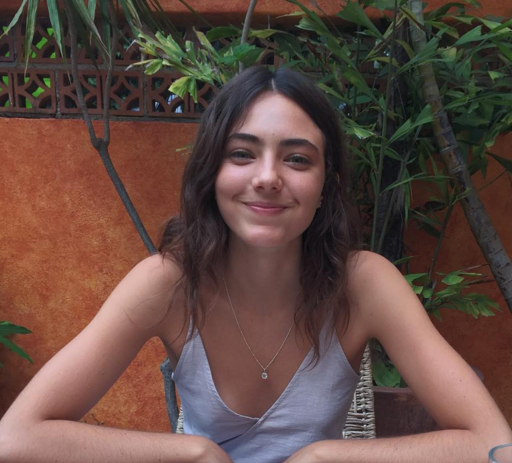
\includegraphics[width=2.5in]{images/expt1/2.png}
	 \caption[GMRT sampling map for an instant ]{\small GMRT sampling map for an instant. The white pixels correspond to locations where fourier data is available}
	\label{fig:expt12}
\end{figure}

\item The star locations are picked uniform randomly and the intensity of each star is chosen uniformly between $[0.3, 1]$. The two color coded original images are shown in Fig. \ref{fig:expt11} with the background sky as black and color of stars varying from blue to red as intensity increases.


\item For both left and right images, Fourier measurements are available as per the GMRT sampling map for an instant consisting of 746 points as shown in Fig. \ref{fig:expt12}.  Thus $\Phi_x = \Phi_y$.

\begin{figure}[t!]
\hspace{-0.5in}
%\begin{center}  \vspace{-0.1in}
\subfigure[Left image]{
	\includegraphics[width=4in]{images/expt1/3a.png}
		}
		\hspace{-1in}
\subfigure[Right image]{
	\includegraphics[width=4in]{images/expt1/3b.png}
		}
\caption [Dirty images, 175 stars, 33\% overlap, 746 points,  rms $1e^{-4}$]{Dirty images, 175 stars, 33\% overlap, 746 points, rms $1e^{-4}$}
\label{fig:expt13}
%\end{center}
\end{figure}


\item We consider additive white gaussian noise with a rms value of $1e^{-4}$.
\item For the initial guesses for $z_x$ and $z_y$ we first find the dirty images by performing a direct Fourier inverse while setting zeros at locations where Fourier data is not available. We then extract the corresponding $z_x$ and $z_y$ which in this case are the images themselves since $\Psi = I$ and use these as starting points. The dirty images are shown in Fig. \ref{fig:expt13}.

\item We choose $\mu = 0$ and $\mu = 0.01$ where in the first case there is no coupling and in the second case coupling is present. We use $\lambda_x = \lambda_y = \lambda$ and vary it in the logarithmic scale between [-3.75, -2.75] in steps of size 0.25. 
\item We terminate the algorithm either when the relative difference in value of objective function is less than $1e^{-7}$ or when we reach 30000 iterations.
\item The relative error vs.  $\lambda$ graphs for the left and right images are shown in Fig. \ref{fig:expt14}.

\vspace{-0.2in}
\begin{figure}[H]

%\begin{center}  \vspace{-0.1in}
\subfigure[Left image]{
	\includegraphics[width=3in]{images/expt1/4a.png}
		}
\hspace{-0.1in}
\subfigure[Right image]{
	\includegraphics[width=3in]{images/expt1/4b.png}
		}
\caption [Error vs $\lambda$, 175 stars, 33\% overlap, 746 points,  rms $1e^{-4}$]{Error vs $\lambda$, 175 stars, 33\% overlap, 746 points, rms $1e^{-4}$}
\label{fig:expt14}
%\end{center}
\end{figure}

\item The reconstructed left and right images for $\lambda = 1e^{-3.25}$ for the two values of $\mu$ are shown in Fig. \ref{fig:expt15} and  Fig. \ref{fig:expt16} respectively. The comparison of the zoomed regions highlighted by the boxes are with corresponding regions from the original images are shown in Fig. \ref{fig:expt17}  and Fig. \ref{fig:expt18}.


\vspace{-0.2in}
\begin{figure}[H]
\hspace{-0.5in}
%\begin{center}  \vspace{-0.1in}
\subfigure[Coupled($\mu = 0.01$) ]{
	\includegraphics[width=4in]{images/expt1/5a.png}
		}
\hspace{-1in}
\subfigure[Separate($\mu = 0$)]{
	\includegraphics[width=4in]{images/expt1/5b.png}
		}		
\caption [Reconstructed left images, 175 stars, 33\% overlap, 746 points,  rms $1e^{-4}$, $\lambda = 1e^{-3.25}$]{Reconstructed left images, 175 stars, 33\% overlap, 746 points, rms $1e^{-4}$, $\lambda = 1e^{-3.25}$}
\label{fig:expt15}
%\end{center}
\end{figure}
\vspace{-0.2in}
\begin{figure}[H]
%\begin{center}  \vspace{-0.1in}
\subfigure[Coupled$(\mu = 0.01)$]{
	\includegraphics[width=2.1in]{images/expt1/7a.png}
		}
\hspace{-0.15in}
\subfigure[Separate$(\mu = 0$)]{
	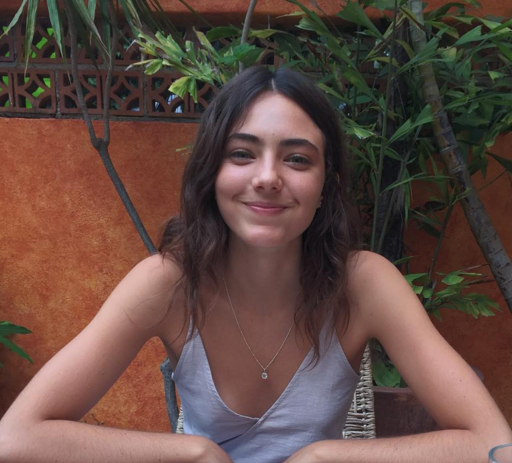
\includegraphics[width=1.9in]{images/expt1/7b.png}
		}
		\hspace{-0.15in}
\subfigure[Original]{
	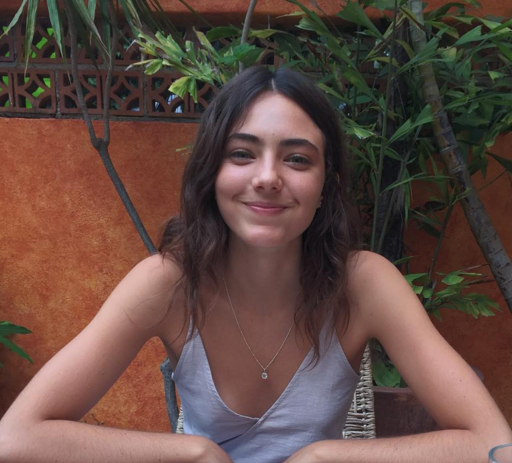
\includegraphics[width=2in]{images/expt1/7c.png}
		}	
\caption [Zoomed left image regions, 175 stars, 33\% overlap, 746 points,  rms $1e^{-4}$, $\lambda = 1e^{-3.25}$]{Zoomed left image regions, 175 stars, 33\% overlap, 746 points, rms $1e^{-4}$, $\lambda = 1e^{-3.25}$ The image using separate formulation has extra blue star near the central red star.}
\label{fig:expt17}
%\end{center}
\end{figure}

\end{enumerate}


\vspace{-0.2in}
\begin{figure}[h!]
\hspace{-0.5in}
%\begin{center}  \vspace{-0.1in}
\subfigure[Coupled($\mu = 0.01$)]{
	\includegraphics[width=4in]{images/expt1/6a.png}
		}
\hspace{-1in}
\subfigure[Separate($\mu = 0$)]{
	\includegraphics[width=4in]{images/expt1/6b.png}
		}		
\caption [Reconstructed right images, 175 stars, 33\% overlap, 746 points,  rms $1e^{-4}$, $\lambda = 1e^{-3.25}$]{Reconstructed right images, 175 stars, 33\% overlap, 746 points, rms $1e^{-4}$, $\lambda = 1e^{-3.25}$}
\label{fig:expt16}
%\end{center}
\end{figure}
\vspace{-0.2in}
\begin{figure}[h!]
%\begin{center}  \vspace{-0.1in}
\subfigure[Coupled$(\mu = 0.01)$]{
	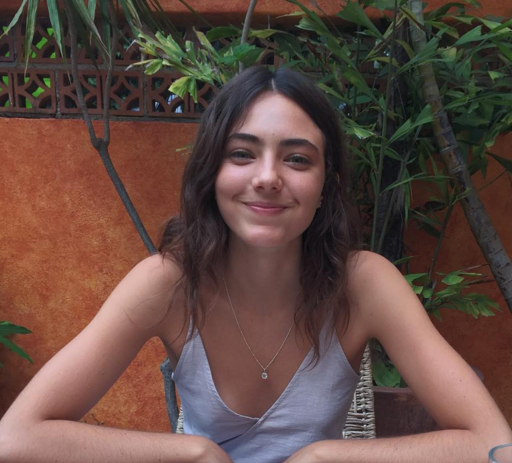
\includegraphics[width=2in]{images/expt1/8a.png}
		}
\hspace{-0.18in}
\subfigure[Separate$(\mu = 0$)]{
	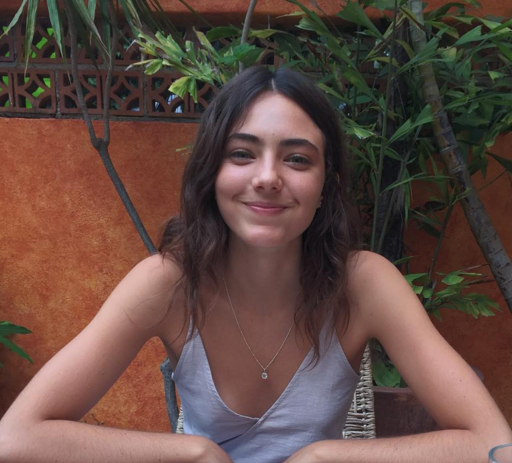
\includegraphics[width=2.1in]{images/expt1/8b.png}
		}
		\hspace{-0.18in}
\subfigure[Original]{
	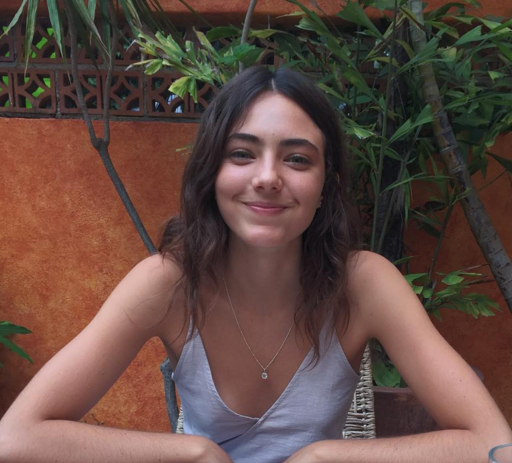
\includegraphics[width=2in]{images/expt1/8c.png}
		}	
\caption [Zoomed right image regions, 175 stars, 33\% overlap, 746 points,  rms $1e^{-4}$, $\lambda = 1e^{-3.25}$]{Zoomed right image regions, 175 stars, 33\% overlap, 746 points, rms $1e^{-4}$, $\lambda = 1e^{-3.25}$.  The image using separate formulation has several excess stars.}
\label{fig:expt18}
%\end{center}
\end{figure}

\subsubsection{Observations}
\begin{enumerate}

\item From Fig. \ref{fig:expt14} we see that the coupled formulation using the alternating algorithm performs better than than the uncoupled formulation. 
\item From Fig. \ref{fig:expt17} and Fig. \ref{fig:expt18} we can see that the reconstructed image in the uncoupled case has both excess stars and missing stars and the coupled formulation not only improves reconstruction in portion of image where overlap occurs but also in regions where there is no overlap.
\item Note that we have a chosen value of $\mu = 0.01$ heuristically since we want to give less weightage to the overlap term as compared to the data fitting terms. 
\item For the best value of $\lambda$ for the left image the error improves from approximately 0.26 to 0.14 and for the right image the error improves from approximately 0.20 to 0.125.
\item Since the level of sparsity in both images and the sampling points are the same in both images both the error and the improvement in error is similar in left and right images.
\end{enumerate}

\subsubsection{Experiment with 50\% overlap}
\begin{enumerate}
\item We repeat the above experiment with same settings except that this time we consider a overlap of 50\%.
\item The new original images are shown in Fig. \ref{fig:expt21}.

\begin{figure}[t!]
\hspace{-0.5in}
%\begin{center}  \vspace{-0.1in}
\subfigure[Left image]{
	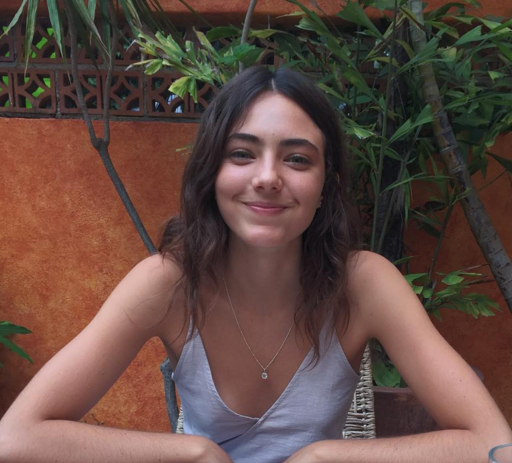
\includegraphics[width=4in]{images/expt1/9a.png}
		}
		\hspace{-1in}
\subfigure[Right image]{
	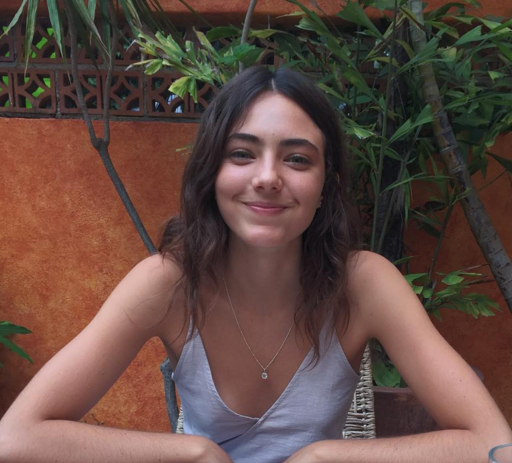
\includegraphics[width=4in]{images/expt1/9b.png}
		}
\caption [Original images, 175 stars, 50\% overlap]{Original left and right images, 175 stars. The last 85 columns of the left image overlap with the first 128 columns of the right image.}
\label{fig:expt21}
%\end{center}
\end{figure}
\item The sampling map, noise rms value, the values of $\mu$ and values of $\lambda$ are same as in the previous experiment.
\item The relative error vs.  $\lambda$ graphs for the left and right images are shown in Fig. \ref{fig:expt22}.

\begin{figure}[b!]

%\begin{center}  \vspace{-0.1in}
\subfigure[Left image]{
	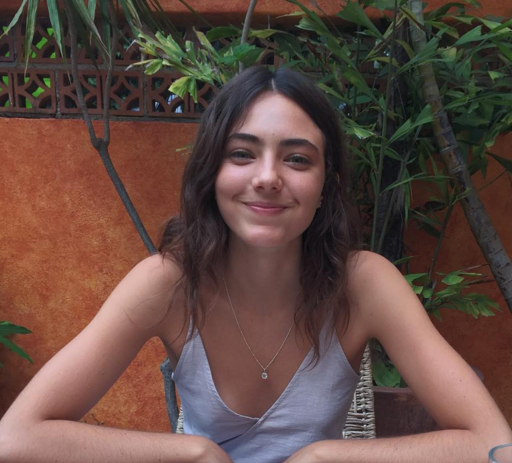
\includegraphics[width=3in]{images/expt1/10a.png}
		}
\hspace{-0.1in}
\subfigure[Right image]{
	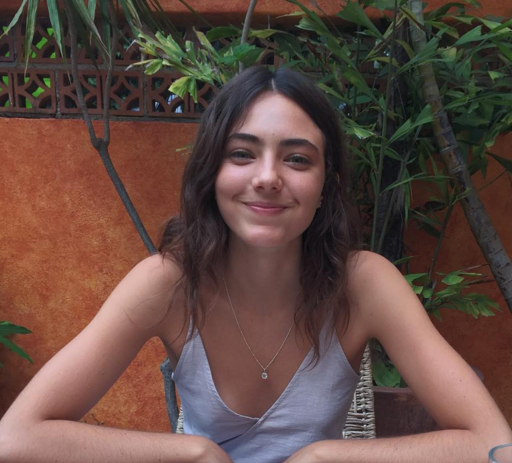
\includegraphics[width=3in]{images/expt1/10b.png}
		}
\caption [Error vs $\lambda$, 175 stars, 50\% overlap, 746 points,  rms $1e^{-4}$]{Error vs $\lambda$, 175 stars, 50\% overlap, 746 points, rms $1e^{-4}$}
\label{fig:expt22}
%\end{center}
\end{figure}

\item The reconstructed left and right images for the best values of $\lambda$ for the two values of $\mu$ are shown in Fig. \ref{fig:expt15} and  Fig. \ref{fig:expt16} respectively. 

\vspace{-0.2in}
\begin{figure}[h!]
\hspace{-0.5in}
%\begin{center}  \vspace{-0.1in}
\subfigure[Coupled, $\mu = 0.01, \lambda = 1e^{-3.5}$]{
	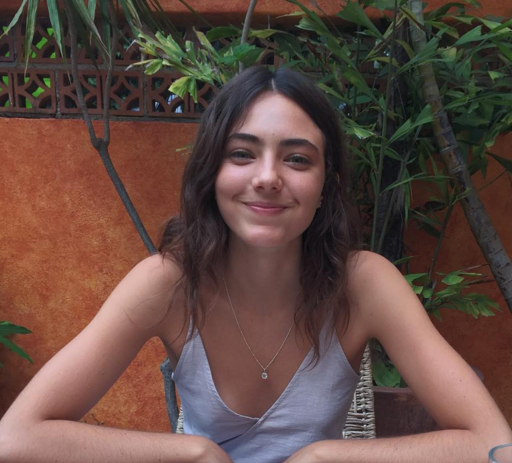
\includegraphics[width=4in]{images/expt1/11a.png}
		}
\hspace{-1in}
\subfigure[Separate, $\mu = 0, \lambda = 1e^{-3.25}$]{
	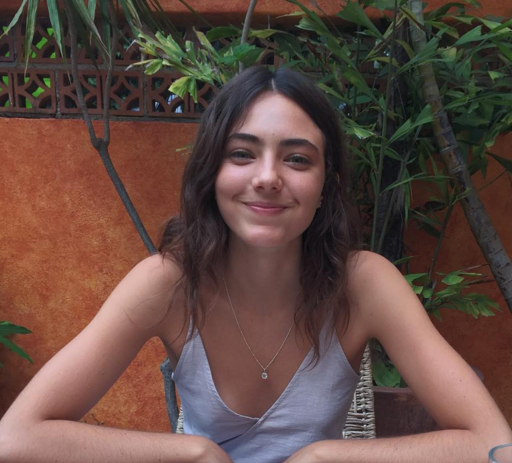
\includegraphics[width=4in]{images/expt1/11b.png}
		}		
\caption [Reconstructed left images, 175 stars, 50\% overlap, 746 points,  rms $1e^{-4}$]{Reconstructed left images, 175 stars, 50\% overlap, 746 points, rms $1e^{-4}$. The image using separate formulation has several excess star in the central region.}
\label{fig:expt15}
%\end{center}
\end{figure}

\begin{figure}[t!]
\hspace{-0.5in}
%\begin{center}  \vspace{-0.1in}
\subfigure[Coupled, $\mu = 0.01, \lambda = 1e^{-3.5}$]{
	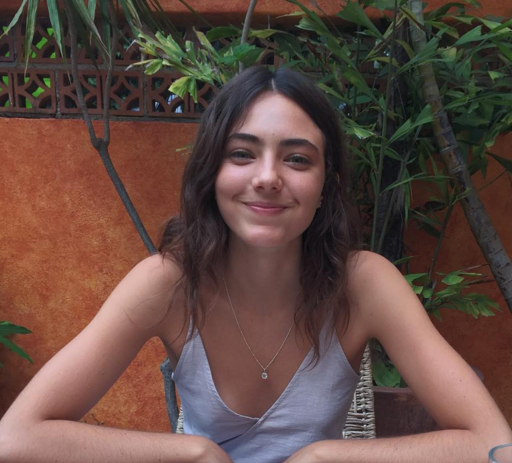
\includegraphics[width=4in]{images/expt1/12a.png}
		}
\hspace{-1in}
\subfigure[Separate, $\mu = 0, \lambda = 1e^{-3.25}$]{
	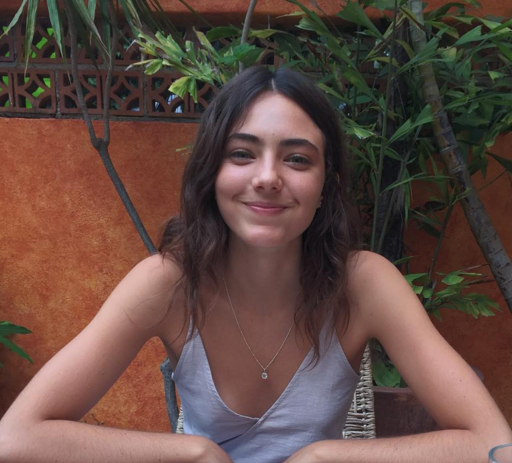
\includegraphics[width=4in]{images/expt1/12b.png}
		}		
\caption [Reconstructed right images, 175 stars, 50\% overlap, 746 points,  rms $1e^{-4}$]{Reconstructed right images, 175 stars, 50\% overlap, 746 points, rms $1e^{-4}$. The image using separate formulation has several excess star in the central region.}
\label{fig:expt16}
%\end{center}
\end{figure}
\end{enumerate}
\subsubsection{Observations}
\begin{enumerate}

\item From Fig. \ref{fig:expt14} and Fig. \ref{fig:expt22} we see that the coupled formulation using the alternating algorithm performs better than than the uncoupled formulation. Also with 50\% overlap the coupled formulation does better than the case where there is 33\% overlap. This is to be expected since with more overlap we have more information and should do better.
\item For the best value of $\lambda$ for the left image the error improves from approximately 0.26 to 0.09 and for the right image the error improves from approximately 0.18 to 0.08.
\item Since the level of sparisity in both images and the sampling points are the same in both images both the error and the improvement in error is similar in left and right images.
\end{enumerate}


\section{Experiments on Shepp-Logan phantom}
\begin{enumerate}
\item In this section we conducted experiments on the Shepp-Logan phantom image, a representative image that is sparse in wavelet domain.
\item We consider the problem in Formulation-3 where the objective function that we wish to minimize is as follows:
 \begin{equation}
 F(z_x, z_y) = \|\Phi_x\Psi z_x - b_x\|_2^2 + \|\Phi_y\Psi z_y - b_y\|_2^2 + \lambda_x \|z_x\|_1 + \lambda_y \|z_y\|_1 + \mu || B_x z_x - B_y z_y||_2^2.
 \end{equation}
 Also since,
\begin{eqnarray}
	x &=& \Psi z_x 	\label{eq:domainx}\\
	y &=& \Psi z_y,
	\label{eq:domainy}
\end{eqnarray}
and our images are sparse in wavelet domain we have $\Psi$ represent an inverse wavelet transform operator.
\item Thus we will first solve for the sparse set of wavelet coefficients and then obtain the reconstructed images using inverse wavelet transform.
\item Since we deal with image sizes of $256 \times 256$ the maximum number of stages we can use is $\log_2(256) = 8$. Also higher the number of stages we use the better sparse approximation we obtain. Thus, we use a 7 stage 2D-DWT with a Haar wavelet to perform the wavelet transform.  In the original images there are approximately 2500 significant coefficients.
\item We will assume that there is an overlap of $S$ pixels between the two reconstructed images and $B_x$ and $B_y$ represent the matrices that take the wavelet coefficients and apply inverse wavelet transform and then extract the portions that will overlap in matching order.
\item The sampling is done by taking slices/lines in the Fourier domain that have equal angular spacing and pass through dc frequency. Thus we have an incomplete set of Fourier measurements obtained by the sampling matrices $\Phi_x$ and $\Phi_y$. We will consider different number lines for the left and right image and observe the performance of the alternating algorithm in this scenario.
\item The Lipschitz constants $L_x$ and $L_y$ are determined as:
\begin{eqnarray}
L_x &=& 2\max(eig( \Phi_x^T \Phi_x))  +  2 \mu \max(eig( B_x^T B_x)) \\
L_y &=& 2\max(eig( \Phi_y^T \Phi_y))  +  2\mu \max(eig( B_y^T B_y))
\end{eqnarray}This value can be upper bounded by $2(1 + \mu)$.
\item The error measure $e$, we use in all our experiments is the relative error and is given by
\begin{equation}
	e = \frac{\|x_r - x\|_F}{\|x \|_F},
\end{equation}
where $x_r$ refers to the reconstructed image and $x$ refers to the original image and $\| \|_F$ refers to the frobenius norm.
\end{enumerate}
We conducted two experiments using the ISTA based alternating algorithm as follows:

\subsubsection{Experiment with 30 and 20 sampling lines}

\begin{enumerate}
\item The left and right original images of size $256 \times 256$ images  in Fig. \ref{fig:expt31} consist of the Shepp-Logan phantom with an overlap between the last 128 columns of the left image with the first 128 columns of the right image. 
\begin{figure}[b!]

%\begin{center}  \vspace{-0.1in}
\hspace{0.4in}
\subfigure[Left image]{
	\includegraphics[width=2.5in]{images/expt3/1a.png}
		}
		\hspace{0.2in}
\subfigure[Right image]{
	\includegraphics[width=2.5in]{images/expt3/1b.png}
		}
\caption [Original images, Shepp-Logan phantom, 50\% overlap]{Original left and right images, Shepp-Logan phantom. The last 128 columns of the left image overlap with the first 128 columns of the right image.}
\label{fig:expt31}
%\end{center}
\end{figure}

\item Fourier data is available at locations given by the sampling map which consist of 30 lines (10501 points) and 20 lines (6657 points) respectively for the left and right image as shown in Fig. \ref{fig:expt32}
\begin{figure}[!t]
\hspace{-0.5in}
%\begin{center}  \vspace{-0.1in}
\subfigure[Left image]{
	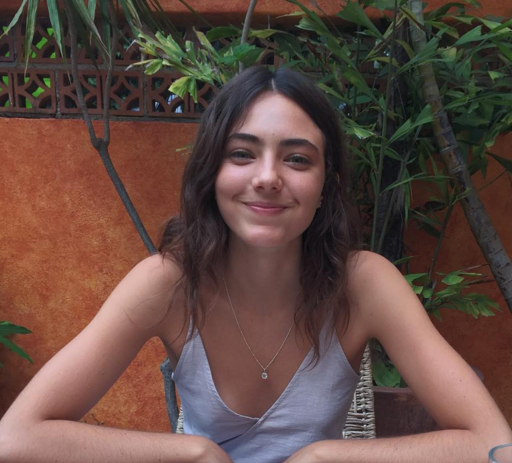
\includegraphics[width=4in]{images/expt3/1c.png}
		}
		\hspace{-1in}
\subfigure[Right image]{
	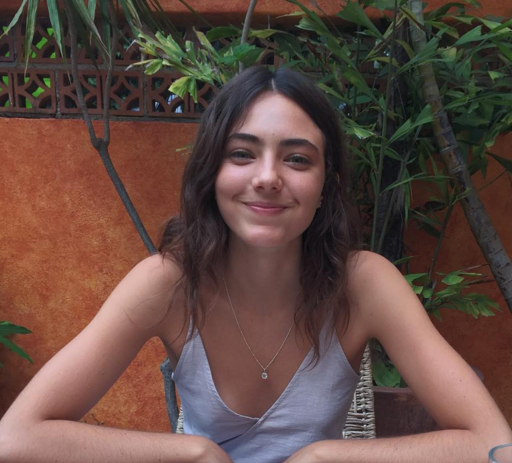
\includegraphics[width=4in]{images/expt3/1d.png}
		}
\caption [Sampling maps, Left 30 lines, Right 20 lines]{Sampling maps, Left 30 lines, Right 20 lines}
\label{fig:expt32}
%\end{center}
\end{figure}

\item We consider additive white gaussian noise with a rms value of $1e^{-4}$.
\item For the initial guesses for $z_x$ and $z_y$ we first find the dirty images by performing a direct Fourier inverse while setting zeros at locations where Fourier data is not available. We then extract the corresponding $z_x$ and $z_y$ which in this case are the wavelet coefficients corresponding to the dirty image and use these as starting points. The dirty images are shown in Fig. \ref{fig:expt33}.

\item We choose $\mu = 0, \mu = 0.01$ and $\mu = 0.1$ where in the first case there is no coupling and in the latter two cases coupling is present. We use $\lambda_x = \lambda_y = \lambda$ and vary it in the logarithmic scale between [-4, -1] in steps of size 0.5. 
\item We terminate the algorithm either when the relative difference in value of objective function is less than $1e^{-7}$ or when we reach 30000 iterations.


\begin{figure}[!b]
\hspace{0.4in}
%\begin{center}  \vspace{-0.1in}
\subfigure[Left image]{
	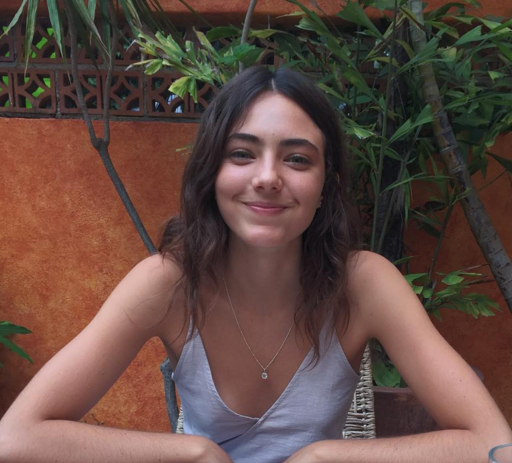
\includegraphics[width=2.5in]{images/expt3/1e.png}
		}
		\hspace{0.2in}
\subfigure[Right image]{
	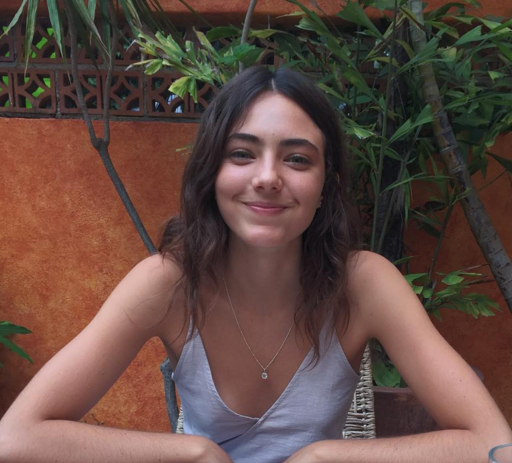
\includegraphics[width=2.5in]{images/expt3/1f.png}
		}
\caption [Dirty images,  Shepp-Logan phantom, Left 30 lines, Right 20 lines, rms $1e^{-4}$]{Dirty images, Shepp-Logan phantom, Left 30 lines, Right 20 lines, rms $1e^{-4}$}
\label{fig:expt33}
%\end{center}
\end{figure}
\item The relative error vs.  $\lambda$ graphs for the left and right images are shown in Fig. \ref{fig:expt34}.

\begin{figure}[H]

%\begin{center}  \vspace{-0.1in}
\subfigure[Left image]{
	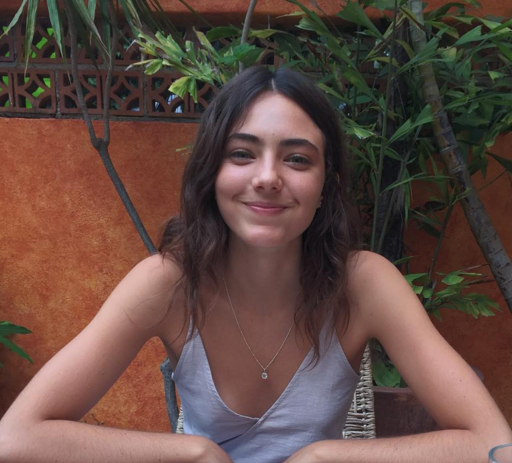
\includegraphics[width=3in]{images/expt3/2a.png}
		}
\hspace{-0.1in}
\subfigure[Right image]{
	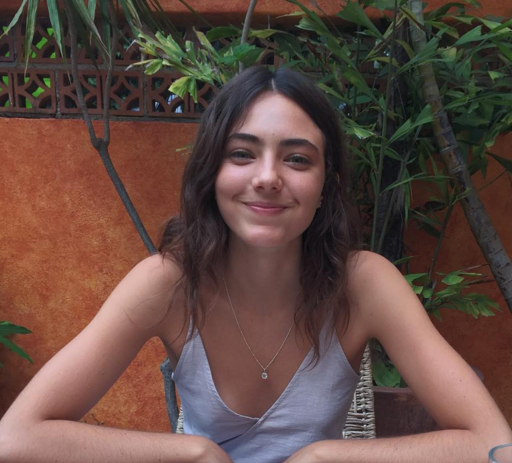
\includegraphics[width=2.9in]{images/expt3/2b.png}
		}
\caption [Error vs $\lambda$, Shepp-Logan phantom, 50\% overlap,  Left 30 lines, Right 20 lines, rms $1e^{-4}$]{Error vs $\lambda$, Shepp-Logan phantom, 50\% overlap,  Left 30 lines, Right 20 lines, rms $1e^{-4}$}
\label{fig:expt34}
%\end{center}
\end{figure}

\item The reconstructed left and right images for $\lambda = 1e^{-3.5}$ for  $\mu  = 0.1 $  and $\lambda = 1e^{-2}$ for  $\mu = 0$ are shown in Fig. \ref{fig:expt35} and  Fig. \ref{fig:expt36} respectively. 

\vspace{-0.2in}
\begin{figure}[t!]
\hspace{0.4in}
%\begin{center}  \vspace{-0.1in}
\subfigure[Coupled, $\mu = 0.01, \lambda = 1e^{-3.5}$]{
	\includegraphics[width=2.5in]{images/expt3/4b.png}
		}
\hspace{0.2in}
\subfigure[Separate, $\mu = 0, \lambda = 1e^{-2}$]{
	\includegraphics[width=2.5in]{images/expt3/4a.png}
		}		
\caption [Reconstructed left images, Shepp-Logan phantom, 50\% overlap,  Left 30 lines, Right 20 lines, rms $1e^{-4}$]{Reconstructed left images, Shepp-Logan phantom, 50\% overlap,  Left 30 lines, Right 20 lines, rms $1e^{-4}$}
\label{fig:expt35}
%\end{center}
\end{figure}

\vspace{-0.2in}
\begin{figure}[b!]
\hspace{0.4in}
%\begin{center}  \vspace{-0.1in}
\subfigure[Coupled, $\mu = 0.01, \lambda = 1e^{-3.5}$]{
	\includegraphics[width=2.5in]{images/expt3/3b.png}
		}
\hspace{0.2in}
\subfigure[Separate, $\mu = 0, \lambda = 1e^{-1.5}$]{
	\includegraphics[width=2.5in]{images/expt3/3a.png}
		}		
\caption [Reconstructed right images, Shepp-Logan phantom, 50\% overlap,  Left 30 lines, Right 20 lines, rms $1e^{-4}$]{Reconstructed right images, Shepp-Logan phantom, 50\% overlap,  Left 30 lines, Right 20 lines, rms $1e^{-4}$. The reconstruction using coupled formulation is visually much better}
\label{fig:expt36}
%\end{center}
\end{figure}
\end{enumerate}
\newpage
\subsubsection{Observations}

\begin{enumerate}
\item From the error graphs and the reconstructed images we observe that for both left and right images the alternating algorithm using the coupled formulation performs better than the uncoupled formulation
\item For the best value of $\lambda$ for the left image the error improves from approximately 0.114 to approximately 0.105 by using coupling and for the right image the error improves from approximately 0.221 to approximately 0.142.
\item For the right image for which we have Fourier data only on 20 sampling lines the improvement is clearly pronounced.
\item This is because the left image has Fourier data available on 30 sampling lines and thus we expect the uncoupled reconstruction of the left image to better than that of the right image. By introducing the coupling term this is transferred into the right image also and we get significant improvement in performance.
\item For the left image the improvement by using the coupled formulation is not as pronounced as that for the right image.
\end{enumerate}

\subsubsection{Experiment with 35 and 25 sampling lines}

\begin{enumerate}
\item We conduct the same experiment as above with the only the sampling maps changed.
\item Fourier data is availabe at locations given by the sampling map which consist of 35 lines (12170 points) and 25 lines (8808 points) respectively for the left and right image as shown in Fig. \ref{fig:expt37}
\begin{figure}[b!]

\hspace{-0.5in}
%\begin{center}  \vspace{-0.1in}
\subfigure[Left image]{
	\includegraphics[width=4in]{images/expt3/5a.png}
		}
		\hspace{-1in}
\subfigure[Right image]{
	\includegraphics[width=4in]{images/expt3/5b.png}
		}
\caption [Sampling maps, Left 35 lines, Right 25 lines]{Sampling maps, Left 35 lines, Right 25 lines}
\label{fig:expt37}
%\end{center}
\end{figure}
\item We choose $\mu = 0, \mu = 0.01$ and $\mu = 0.1$ where in the first case there is no coupling and in the latter two cases coupling is present. We use $\lambda_x = \lambda_y = \lambda$ and vary it in the logarithmic scale between [-4, -2] in steps of size 0.5. 

\begin{figure}[h!]

\vspace{-0.2in}
%\begin{center}  \vspace{-0.1in}
\subfigure[Left image]{
	\includegraphics[width=3in]{images/expt3/6a.png}
		}
\hspace{-0.1in}
\subfigure[Right image]{
	\includegraphics[width=3in]{images/expt3/6b.png}
		}
\caption [Error vs $\lambda$, Shepp-Logan phantom, 50\% overlap,  Left 35 lines, Right 25 lines, rms $1e^{-4}$]{Error vs $\lambda$, Shepp-Logan phantom, 50\% overlap,  Left 35 lines, Right 25 lines, rms $1e^{-4}$}
\label{fig:expt38}
%\end{center}
\end{figure}
\item The relative error vs.  $\lambda$ graphs for the left and right images are shown in Fig. \ref{fig:expt38}.
\item The reconstructed left and right images for $\lambda = 1e^{-3.5}$ for  $\mu  = 0.1 $  and $\lambda = 1e^{-2}$ for  $\mu = 0$ are shown in Fig. \ref{fig:expt39} and  Fig. \ref{fig:expt310} respectively. 


\begin{figure}[b!]
\hspace{0.4in}
%\begin{center}  \vspace{-0.1in}
\subfigure[Coupled, $\mu = 0.01, \lambda = 1e^{-3.5}$]{
	\includegraphics[width=2.5in]{images/expt3/7a.png}
		}
\hspace{0.2in}
\subfigure[Separate, $\mu = 0, \lambda = 1e^{-2}$]{
	\includegraphics[width=2.5in]{images/expt3/7b.png}
		}		
\caption [Reconstructed left images, Shepp-Logan phantom, 50\% overlap,  Left 35 lines, Right 25 lines, rms $1e^{-4}$]{Reconstructed left images, Shepp-Logan phantom, 50\% overlap,  Left 35 lines, Right 25 lines, rms $1e^{-4}$}
\label{fig:expt39}
%\end{center}
\end{figure}


\begin{figure}[t!]
\hspace{0.4in}
%\begin{center}  \vspace{-0.1in}
\subfigure[Coupled, $\mu = 0.01, \lambda = 1e^{-3.5}$]{
	\includegraphics[width=2.5in]{images/expt3/8a.png}
		}
\hspace{0.2in}
\subfigure[Separate, $\mu = 0, \lambda = 1e^{-1.5}$]{
	\includegraphics[width=2.5in]{images/expt3/8b.png}
		}		
\caption [Reconstructed right images, Shepp-Logan phantom, 50\% overlap,  Left 35 lines, Right 25 lines, rms $1e^{-4}$]{Reconstructed right images, Shepp-Logan phantom, 50\% overlap,  Left 35 lines, Right 25 lines, rms $1e^{-4}$. The reconstruction using the coupled framework is better than the other.}
\label{fig:expt310}
%\end{center}
\end{figure}
\end{enumerate}

\subsubsection{Observations}

\begin{enumerate}
\item From the error graphs and the reconstructed images we observe that for both left and right images the alternating algorithm using the coupled formulation performs better than the uncoupled formulation
\item For the best value of $\lambda$ for the left image the error improves from approximately 0.081 to 0.071 by using coupling and for the right image the error improves from approximately 0.152 to 0.094.
\item Again for the right image the improvement is more pronounced than that for the left image due to the fact that for the left image we have Fourier data on 35 sampling lines and for the right image we have Fourier data only on 25 sampling lines.
\item   Since we expect the higher number of samples for the left image to lead to a better reconstruction in the uncoupled formulation, this higher quality is transferred to the right image when we introduce coupling.
\item Comparing the relative error graphs in Fig. \ref{fig:expt38} and Fig. \ref{fig:expt34} we observe that the percentage improvement in the error reduces as data at higher number of Fourier points is available. This conforms with the intuition that if we have almost all Fourier measurements, then we expect both the coupled and uncoupled formulation to perform almost similarly. 
\item We will not deal with radio astronomical extended sources separately in this section but instead will combine the extended sources with point sources and investigate them in the next section.
\end{enumerate}


\section{Experiments on images containing both point and extended sources}
\begin{enumerate}
\item In this section we consider images that consist of both point and extended sources. It is unlikely to find a region of the sky with extended sources alone and most likely we will find extended sources along with point sources in the background. In this case our image will not be sparse in any one domain and we must come up with an alternate formulation to reconstruct such images from incomplete fourier data.
\item Let $J$ be the image containing both point sources and extended sources. We can view $J$ as the sum of two images $J_s$ and $J_w$ where, $J_s$ refers to the image of point source and is sparse in spatial domain and $J_w$ refers to image containing the extended source and is sparse in wavelet domain. An example of such a decomposition is given in Fig. \ref{fig:expt41}.
\item We have,
\begin{eqnarray}
J_w &=& W u \\
J_s &=& I v,
\end{eqnarray}
where  $u$ denotes the wavelet coefficieints, $v$ denotes the pixel values, $W$ refers to the matrix representing the inverse wavelet transform and $I$ refers to the identity matrix.
\begin{figure}[b!]
\hspace{0.4in}
%\vspace{-0.2in}
%\begin{center}  \vspace{-0.1in}
\subfigure[Complete image]{
	\includegraphics[width=1.7in]{images/expt4/1a.png}
		}
\hspace{0.1in}
\subfigure[Spatial domain sparse]{
	\includegraphics[width=1.7in]{images/expt4/1b.png}
		}
		\hspace{0.1in}
\subfigure[Wavelet sparse]{
	\includegraphics[width=1.7in]{images/expt4/1c.png}
		}
\caption [Decomposition of image containing both point and extended sources]{Decomposition of image containing both point and extended sources}
\label{fig:expt41}
%\end{center}
\end{figure}
\item Thus we have,
\begin{equation}
	J = W u + I v.
\end{equation} 
\item Now let us consider a setting as before where we have two images with some information overlap. Let the lexicographic ordering of the left image be denoted by $x$ of size $N \times 1$ and that of the right image by denoted by $y$ of size $N \times 1$. Then,
\begin{eqnarray}
	x &=& Wu_x + Iv_x \\
	y  &=& Wu_y + Iv_y	
\end{eqnarray}
\item We have Fourier measurements $b_x$ and $b_y$ using the sampling matrices $\Phi_x$ and $\Phi_y$ where,
	\begin{eqnarray}
  b_x &=& \Phi_x x  + n_x\\
  b_y   &=& \Phi_y y + n_y,
  \end{eqnarray}
 where $\Phi_x$ and $\Phi_y$ are $M_x \times N$ and $M_y \times N$ measurement matrices respectivley and $n_x$ and $n_y$ are terms corresponding to the noise added to the system while obtaining the measurements ($M_x < N, \ M_y < N)$.
 
\item Let $f_x$ and $f_y$ be the $S \times 1$ feature vectors obtained from $x$ and $y$ as,
\begin{eqnarray}
f_x &=& B_x u_x + C_x v_x\\
f_y &=& B_y u_y + C_y v_y,
\label{eq:mix}
\end{eqnarray}
where $B_x, B_y, C_x$ and $C_y$ are feature extraction matrices.

\item Then along the lines of Formulation-3 we will find $u_x^*, v_x^*, u_y^* and v_y^*$ by performing joint minimization of the cost function $G(u_x, v_x, u_y, v_y)$ as follows:
 \begin{equation}
u_x^*, v_x^*, u_y^*, v_y^* = \arg \min_{u_x, v_x, u_y, v_y} G(u_x, v_x, u_y, v_y)
 \end{equation}
where,
 \begin{eqnarray}
G(u_x, v_x, u_y, v_y) &\equiv& \|\Phi_x\Psi u_x + \Phi v_x - b_x\|_2^2 + \|\Phi_y\Psi u_y +\Phi v_y  - b_y\|_2^2 + \lambda^s_x \|u_x\|_1 + \lambda^w_x \|v_x\|_1 \nonumber \\
& & +  \lambda^s_y \|u_y\|_1 + \lambda^w_y \|v_y\|_1   + \mu ||f_x - f_y||_2^2.
\label{eq:cstf}
 \end{eqnarray}
\item Here $\lambda^s_x$ and $\lambda^s_y$ are weights to the spatial domain sparse component of the reconstructed image while $\lambda^w_x$ and $\lambda^w_y$ are weights to the wavelet domain sparse component. In general these can be different since we may have a different level of sparsity in the two domains.
\item We will make the simplifying assumption and choose $\lambda^s_x = \lambda^w_x = \lambda_x$ and $\lambda^s_y = \lambda^w_y = \lambda_y$.
\item Under this assumption we can express the above minimization problem using Formulation-3 where,
\begin{align}
z_x &= \begin{bmatrix}
u_x \\
v_x
\end{bmatrix}\\
z_y &= \begin{bmatrix}
u_y \\
v_y
\end{bmatrix}\\
A_x &= \begin{bmatrix}
\Phi_x\Psi &  \Phi_x
\end{bmatrix}\\
A_y &= \begin{bmatrix}
\Phi_y\Psi &  \Phi_y
\end{bmatrix}\\
D_x &= \begin{bmatrix}
B_x &  0 \\
0 & C_x
\end{bmatrix}\\
D_y &= \begin{bmatrix}
B_y &  0 \\
0 & C_y
\end{bmatrix}
\end{align}
\item Thus we will first find $z_x^*$ and $z_y^*$ by solving the joint minimization problem,
 \begin{equation}
 z_x^*, z_y^* = \arg \min_{z_x, z_y} F(z_x, z_y),
 \end{equation}
where,
 \begin{equation}
 F(z_x, z_y) \equiv \|A_x z_x - b_x\|_2^2 + \|A_y z_y - b_y\|_2^2 + \lambda_x \|z_x\|_1 + \lambda_y \|z_y\|_1 + \mu ||D_x z_x - D_y z_y||_2^2.
 \end{equation}
\end{enumerate}
We conduct three classes of experiments with this formulation,
\begin{enumerate}
\item Experiment to confirm the need of a better description for images consisting of both point and extended sources
\item Images consisting of both the Shepp-Logan phantom and point sources. The Shepp-Logan phantom is a prime example of a wavelet sparse image and hence we use this to test our framework.
\item Images consisting of both astronomical point sources and astronomical extended sources.
\end{enumerate}

\subsection{Experiment to confirm need for better description}

\begin{enumerate}
\item In this experiment we will consider a single image reconstruction problem where the image consists of a spatial domain sparse component and a wavelet domain sprase component. We will perform the reconstruction using both the formulation presented above and a formulation that considers the image only to be wavelet sparse. In both cases we will make use of the FISTA algorithm to perform the reconstruction. It is clear that a formulation that considers the image to be sparse in spatial domain will certainly not work so we dont consider that case.
\item We construct the original image by adding 100 stars at random locations in the background of the Shepp-Logan phantom image as shown in Fig. \ref{fig:expt42}. Each star is of size $2\times2$ pixels and has uniform intensity value of 1.

 \begin{figure}[t!]
	\centering \vspace{-0.1in}
	\includegraphics[width=2.5in]{images/expt4/2.png}
	 \caption[Original image, Shepp-Logan phantom, 100 stars ]{\small Original image, Shepp-Logan phantom, 100 stars}
	\label{fig:expt42}
\end{figure}


\item We have Fourier data according to the sampling map consisting of 35 sampling lines (12170 points points) as shown in Fig. \ref{fig:expt43}.
 \begin{figure}[t!]
	\centering 
	\includegraphics[width=2.2in]{images/expt4/3.png}
	 \caption[Sampling map, 35 lines ]{\small Sampling map, 35 lines}
	\label{fig:expt43}
\end{figure}
\item We assume that there is no noise.
\item The Lipschitz constants $L$ is determined as:
\begin{eqnarray}
L &=& 2\max(eig( A^T A) 
\end{eqnarray}
This value can be upper bounded by $4$.
\item The value of $\lambda$ is varied in the logarithmic scale between [-4, 0] in steps of 0.5.
 \begin{figure}[b!]
	\centering \vspace{-0.1in}
	\includegraphics[width=2.5in]{images/expt4/4.png}
	 \caption[Dirty image, Shepp-Logan phantom, 100 stars, 35 lines ]{\small Dirty image, Shepp-Logan phantom, 100 stars, 35 lines}
	\label{fig:expt44}
\end{figure}
\item From the dirty image (Fig. \ref{fig:expt44}) it is not easy to recover the coefficients of the wavelet domain sparse and spatial domain sparse component. But since our algorithm is insensitive to starting point we initialize both sets of coefficients with the corresponding coefficients derived from the combined image.


\item The error vs $\lambda$ plot for the two formulations is shown in Fig. \ref{fig:expt45}.

 \begin{figure}[t!]
	\centering \vspace{-0.1in}
	\includegraphics[width=3.5in]{images/expt4/5.png}
	 \caption[Error vs $\lambda$, Shepp-Logan phantom, 100 stars, 35 lines ]{\small Error vs $\lambda$, Shepp-Logan phantom, 100 stars, 35 lines}
	\label{fig:expt45}
\end{figure}


\item The reconstructed image for the best value of $\lambda$ using the formulation presented above and the formulation that assumes the image to be sparse in wavelet domain alone is shown in Fig. \ref{fig:expt46}.
\begin{figure}[b!]
\hspace{0.4in}
%\begin{center}  \vspace{-0.1in}
\subfigure[Sum of wavelet sparse and spatial domain sparse, $\lambda = 1e^{-2}$]{
	\includegraphics[width=2.5in]{images/expt4/6a.png}
		}
\hspace{0.2in}
\subfigure[Wavelet domain sparse only, $\lambda = 1e^{-2}$]{
	\includegraphics[width=2.5in]{images/expt4/6b.png}
		}		
\caption [Reconstructed images, Shepp-Logan phantom, 100 stars]{Reconstructed images, Shepp-Logan phantom, 100 stars. The reconstruction of the phantom is better in the left image}
\label{fig:expt46}
%\end{center}
\end{figure}


\item The spatial domain sparse component and the wavelet domain sparse component of the reconstruction using the new formulation is shown in Fig. \ref{fig:expt47}.
\begin{figure}[t!]
\hspace{0.4in}
%\begin{center}  \vspace{-0.1in}
\subfigure[Spatial domain sparse]{
	\includegraphics[width=2.5in]{images/expt4/7a.png}
		}
\hspace{0.2in}
\subfigure[Wavelet domain sparse]{
	\includegraphics[width=2.5in]{images/expt4/7b.png}
		}		
\caption [Reconstructed image decompositions, Shepp-Logan phantom, 100 stars, $\lambda = 1e^{-2}$ ]{Reconstructed image decompositions, Shepp-Logan phantom, 100 stars, $\lambda = 1e^{-2}$}
\label{fig:expt47}
%\end{center}
\end{figure}
\end{enumerate}


\subsubsection{Observations}
\begin{enumerate}
\item The formulation that assumes the image to be only wavelet sparse performs much worse than the formulation that considers the image to have both a spatial domain sparse component and a wavelet domain sparse component.
\item The spatial domain sparse component of the reconstructed image consists of not only the point sources but also parts of the edges of the Shepp-Logan phantom. This is to be expected since the edges have high contribution to the wavelet coefficients in the wavelet domain sparse image.
\item The wavelet domain sparse component contains the Shepp-Logan phantom and also a few stray stars.
\item Thus we need the formulation presented above to tackle images that contain both a spatial domain sparse component and a wavelet domain sparse component.
\end{enumerate}

\subsection{Experiments on images of Shepp-Logan phantom along with stars}
In this section we will use the formulation above to reconstruct left and right images where there is information overlap between the two images. We compare the performance of the cases where we do joint minimization using the alternating algorithms with the case where we solve for left and right images separately. By decomposing the image into two components (a wavelet domain sparse component and a spatial domain sparse component) we are effectively increasing the size of the problem by a factor of 2 and to obtain faster run times we use the FISTA variant of the alternating algorithm.
\subsubsection{Experiment with 40 sampling lines for both images}
\begin{enumerate}
\item The left image is constructed as follows. We start with the Shepp-Logan phantom and add 200 stars at random locations in the background. Each star is of size $2 \times 2$ pixels and has intensity value of 1.
\item For the right image, we start with the same Shepp-Logan phantom image and add 200 stars in different random locations as compared to the left image. The two original images are shown in Fig. \ref{fig:expt51}.
\item Thus the two images can be viewed as having a common wavelet sparse component and different spatial domain sparse components.
\begin{figure}[b!]
\hspace{0.4in}
%\begin{center}  \vspace{-0.1in}
\subfigure[Left image]{
	\includegraphics[width=2.5in]{images/expt5/1a.png}
		}
		\hspace{0.2in}
\subfigure[Right image]{
	\includegraphics[width=2.5in]{images/expt5/1b.png}
		}
\caption [Original images, Shepp-Logan phantom, 200 stars]{Original images, Shepp-Logan phantom, 200 stars. Only the star locations in both images are different}
\label{fig:expt51}
%\end{center}
\end{figure}

\item Fourier data is available at locations given by the sampling map which consist of 40 lines (13387 points) for voth the left and right image as shown in Fig. \ref{fig:expt52}
\begin{figure}[!t]

\begin{center}  \vspace{-0.1in}

\includegraphics[width=2.5in]{images/expt5/2.png}

\caption [Sampling map, 40 lines]{Sampling map, 40 lines}
\label{fig:expt52}
\end{center}
\end{figure}

\item We consider the noiseless case. The information overlap present is that the wavelet sparse component of both images must be the same. Thus in Eq. \ref{eq:mix}, we have, $B_x = W, C_x = 0, B_y = W$ and $C_y = 0$ where $W$ is the inverse wavelet transform operator. 
\item From the dirty images (Fig. \ref{fig:expt53}) it is not easy to recover the coefficients of the wavelet domain sparse and spatial domain sparse component. But since our algorithm is insensitive to starting point we initialize both sets of coefficients with the corresponding coefficients derived from the combined images.

\begin{figure}[!b]
\hspace{0.4in}
%\begin{center}  \vspace{-0.1in}
\subfigure[Left image]{
	\includegraphics[width=2.5in]{images/expt5/3a.png}
		}
		\hspace{0.2in}
\subfigure[Right image]{
	\includegraphics[width=2.5in]{images/expt5/3b.png}
		}
\caption [Dirty images,  Shepp-Logan phantom, 200 stars, 40 lines]{Dirty images,  Shepp-Logan phantom, 200 stars, 40 lines}
\label{fig:expt53}
%\end{center}
\end{figure}

\item We choose $\mu = 0$ and $\mu = 0.1$ where in the first case there is no coupling and in the latter case coupling is present. We use $\lambda_x = \lambda_y = \lambda$ and vary it in the logarithmic scale between [-5.5, -3] in steps of size 0.5. 
\item The Lipschitz constant in this case can be upper bounded by $2(2 + \mu)$.
\item We terminate the algorithm either when the relative difference in value of objective function is less than $1e^{-7}$ or when we reach 20000 iterations.


\item The relative error vs.  $\lambda$ graphs for the left and right images are shown in Fig. \ref{fig:expt54}.

\begin{figure}[H]

%\begin{center}  \vspace{-0.1in}
\subfigure[Left image]{
	\includegraphics[width=3.2in]{images/expt5/4a.png}
		}
\hspace{-0.1in}
\subfigure[Right image]{
	\includegraphics[width=3.2in]{images/expt5/4b.png}
		}
\caption [Error vs $\lambda$, Shepp-Logan phantom, 200 stars,  40 lines]{Error vs $\lambda$, Shepp-Logan phantom, 200 stars,  40 lines]}
\label{fig:expt54}
%\end{center}
\end{figure}

\item The reconstructed left and right images for $\lambda = 1e^{-5}$ for  $\mu  = 0.1 $  and $\lambda = 1e^{-5}$ for  $\mu = 0$ are shown in Fig. \ref{fig:expt55} and  Fig. \ref{fig:expt56} respectively. 

\vspace{-0.2in}
\begin{figure}[H]
\hspace{0.4in}
%\begin{center}  \vspace{-0.1in}
\subfigure[Coupled, $\mu = 0.1, \lambda = 1e^{-5}$]{
	\includegraphics[width=2.5in]{images/expt5/5a.png}
		}
\hspace{0.2in}
\subfigure[Separate, $\mu = 0, \lambda = 1e^{-5}$]{
	\includegraphics[width=2.5in]{images/expt5/5b.png}
		}		
\caption [Reconstructed left images, Shepp-Logan phantom, 200 stars, 40 lines]{Reconstructed left images, Shepp-Logan phantom, 200 stars, 40 lines. The reconstruction of the phantom is visibly better in the coupled formulation.}
\label{fig:expt55}
%\end{center}
\end{figure}


\begin{figure}[H]
\hspace{0.4in}
%\begin{center}  \vspace{-0.1in}
\subfigure[Coupled, $\mu = 0.1, \lambda = 1e^{-5}$]{
	\includegraphics[width=2.5in]{images/expt5/6a.png}
		}
\hspace{0.2in}
\subfigure[Separate, $\mu = 0, \lambda = 1e^{-5}$]{
	\includegraphics[width=2.5in]{images/expt5/6b.png}
		}		
\caption [Reconstructed right images, Shepp-Logan phantom, 200 stars, 40 lines]{Reconstructed right images, Shepp-Logan phantom, 200 stars, 40 lines. The reconstruction of the phantom is visibly better in the coupled formulation.}
\label{fig:expt56}
%\end{center}
\end{figure}
\end{enumerate}
\subsubsection{Observations}
\begin{enumerate}
\item From the error graphs and the reconstructed images we observe that for both left and right images the alternating algorithm using the coupled formulation performs better than the uncoupled formulation
\item For the best value of $\lambda$ for the left image the error improves from approximately 0.102 to 0.056 by using coupling and for the right image the error improves from approximately 0.105 to 0.056.
\item Since the level of sparsity in both images and the sampling points are the same in both images both the error and the improvement in error are similar in left and right images.
\end{enumerate}

We also performed the experiment where the sampling map for the left image consisted of 40 sampling lines and that of the right image consisted of 30 sampling lines. In this case, we observed that the improvement in the reconstruction of the right image which has fewer number of sampling points is much higher than that in the reconstruction of the left image. This is due to the fact that for the right image, the uncoupled formulation performs much worse as compared to for the left image since it has Fourier data available at much fewer points.
%
%\subsubsection{Experiment with 40 sampling lines for left image and 30 sampling lines for the right image}
%\begin{enumerate}
%\item We repeat the above experiment but this time we consider the case where Fourier data is available on 40 sampling lines for the left image and only on 30 sampling lines for the right image.
%\item The original images in this case will have stars at different random locations as compared to the previous experiment but we keep rest of the parameters and settings the same as in the above experiment.
%\item The relative error vs.  $\lambda$ graphs for the left and right images are shown in Fig. \ref{fig:expt57}.
%
%\begin{figure}[H]
%
%%\begin{center}  \vspace{-0.1in}
%\subfigure[Left image]{
%	\includegraphics[width=3.2in]{images/expt5/7a.png}
%		}
%\hspace{-0.1in}
%\subfigure[Right image]{
%	\includegraphics[width=3.2in]{images/expt5/7b.png}
%		}
%\caption [Error vs $\lambda$, Shepp-Logan phantom, 200 stars,  Left 40 lines, Right 30 lines]{Error vs $\lambda$, Shepp-Logan phantom, 200 stars,  Left 40 lines, Right 30 lines]}
%\label{fig:expt57}
%%\end{center}
%\end{figure}
%
%\item The reconstructed left and right images for $\lambda = 1e^{-5}$ for  $\mu  = 0.1 $  and $\lambda = 1e^{-5}$ for  $\mu = 0$ are shown in Fig. \ref{fig:expt58} and  Fig. \ref{fig:expt59} respectively. 
%
%\vspace{-0.2in}
%\begin{figure}[H]
%
%%\begin{center}  \vspace{-0.1in}
%\subfigure[Coupled, $\mu = 0.1, \lambda = 1e^{-5}$]{
%	\includegraphics[width=2.5in]{images/expt5/8a.png}
%		}
%\hspace{0.2in}
%\subfigure[Separate, $\mu = 0, \lambda = 1e^{-5}$]{
%	\includegraphics[width=2.5in]{images/expt5/8b.png}
%		}		
%\caption [Reconstructed left images, Shepp-Logan phantom, 200 stars, Left 40 lines,  Right 30 lines]{Reconstructed left images, Shepp-Logan phantom, 200 stars, Left 40 lines,  Right 30 lines}
%\label{fig:expt58}
%%\end{center}
%\end{figure}
%
%
%\begin{figure}[H]
%
%%\begin{center}  \vspace{-0.1in}
%\subfigure[Coupled, $\mu = 0.1, \lambda = 1e^{-5}$]{
%	\includegraphics[width=2.5in]{images/expt5/9a.png}
%		}
%\hspace{0.2in}
%\subfigure[Separate, $\mu = 0, \lambda = 1e^{-5}$]{
%	\includegraphics[width=2.5in]{images/expt5/9b.png}
%		}		
%\caption [Reconstructed right images, Shepp-Logan phantom, 200 stars, Left 40 lines,  Right 30 lines]{Reconstructed right images, Shepp-Logan phantom, 200 stars, Left 40 lines,  Right 30 lines}
%\label{fig:expt59}
%%\end{center}
%\end{figure}
%\end{enumerate}
%\subsubsection{Observations}
%\begin{enumerate}
%\item From the error graphs and the reconstructed images we observe that for both left and right images the alternating algorithm using the coupled formulation performs better than the uncoupled formulation
%\item For the best value of $\lambda$ for the left image the error improves from approximately 0.10 to 0.06 by using coupling and for the right image the error improves from approximately 0.20 to 0.08.
%\item For the right image the improvement is more pronounced than that for the left image due to the fact that for the left image we have Fourier data on 40 sampling lines and for the right image we have Fourier data only on 30 sampling lines.
%\item  Thus the gains of using the coupled formulation are much higher when we have higher number of samples for one image and lower number of samples for the other image. In this case, the reconstruction of the image with the lower number of samples is improved significantly.
%\end{enumerate}
In the next section, we will consider images of extended astronomical sources along with point sources and conduct experiments to investigate the performance using the coupled formulation.

\subsection{Experiment on images containing astronomical extended and point sources}
In this section we will explore the case where a large difference in the number of sampling points present in the left and right images may lead to loss in performance in the image with the higher number of samples while using the coupled framework.
We will refer to this problem as the ``difference in sampling points problem'' and will subsequently present 3 different ways to tackle this problem.
\begin{enumerate}
\item The original left and right images shown in Fig. \ref{fig:expt61} and consist of an extended source along with 200 stars.
There is an overlap of 128 columns between the two images.
\item The stars are of size $2 \times 2$ and have intensity values in range [0.3, 1] picked uniform randomly.
\item Fourier data is available at the sampling maps generated by the GMRT array using aperture synthesis as shown in Fig. \ref{fig:expt62}.

\item For the left image, we consider sampling map generated by aperture synthesis for 12 hours with a sample collected every 10 minutes.
\item For the left image, we consider sampling map generated by aperture synthesis for 12 hours with a sample collected every 30 minutes.
\item There is a large difference in the number of points in the sampling map of the left and right images. The left sampling map has 23884 points while the right sampling map has 11192.
\begin{figure}[h!]
\hspace{0.4in}
%\begin{center}  \vspace{-0.1in}
\subfigure[Left image]{
	\includegraphics[width=2.5in]{images/expt6/1a.png}
		}
		\hspace{0.2in}
\subfigure[Right image]{
	\includegraphics[width=2.5in]{images/expt6/1b.png}
		}
\caption [Original images, Extended source, 200 stars]{Original images, Extended source , 200 stars. Overlap of 128 columns}
\label{fig:expt61}
%\end{center}
\end{figure}

\begin{figure}[h!]

\hspace{0.4in}
%\begin{center}  \vspace{-0.1in}
\subfigure[Left image, Sampling period = 10 min]{
	\includegraphics[width=2.5in]{images/expt6/2a.png}
		}
		\hspace{0.2in}
\subfigure[Right image, Sampling period = 30 min]{
	\includegraphics[width=2.5in]{images/expt6/2b.png}
		}
\caption [Sampling maps, Duration = 12h]{Sampling maps, Duration = 12h}
\label{fig:expt62}
%\end{center}
\end{figure}

\item The extended source forms the wavelet sparse component (approx. 3700 significant coefficients) of our image and the stars form the spatial domain sparse component. A coefficient is said to be significant if it is more than 0.5\% of maximum coefficient value.

\item The information overlap that we assume is that the last 128 columns of the wavelet sparse component of the left image match with the first 128 columns of the wavelet sparse component of the right image.
\item We could in general assume overlap for the spatial domain sparse components too but we do not consider this.
\item We consider the noiseless case. We initialize both sets of coefficients with the corresponding coefficients derived from the dirty images shown in Fig. \ref{fig:expt63}.
%\begin{center}  \vspace{-0.1in}

\begin{figure}[h!]
\hspace{0.4in}
\subfigure[Left image, Sampling period = 10 min]{
	\includegraphics[width=2.5in]{images/expt6/3a.png}
		}
		\hspace{0.2in}
\subfigure[Right image, Sampling period = 30 min]{
	\includegraphics[width=2.5in]{images/expt6/3b.png}
		}
\caption [Dirty images, Extended source, 200 stars, Duration 12h]{Dirty images, Extended source , 200 stars, Duration 12h}
\label{fig:expt63}
%\end{center}
\end{figure}


\item We choose $\mu = 0$ and $\mu = 0.1$ where in the first case there is no coupling and in the latter case coupling is present. We use $\lambda_x = \lambda_y = \lambda$ and vary it in the logarithmic scale between [-6, -2] in steps of size 0.5. 
\item The Lipschitz constant in this case can be upper bounded by $2(2 + \mu)$.
\item We terminate the algorithm either when the relative difference in value of objective function is less than $1e^{-7}$ or when we reach 20000 iterations.
\item The relative error vs.  $\lambda$ graphs for the left and right images are shown in Fig. \ref{fig:expt64}.

\begin{figure}[h!]

%\begin{center}  \vspace{-0.1in}
\subfigure[Left image]{
	\includegraphics[width=3.2in]{images/expt6/4a.png}
		}
\hspace{-0.1in}
\subfigure[Right image]{
	\includegraphics[width=3.2in]{images/expt6/4b.png}
		}
\caption [Error vs $\lambda$, Extended source, 200 stars,  Duration = 12h, Left sampling period = 10 min, Right sampling period = 30 min]{Error vs $\lambda$, Extended source, 200 stars,  Duration = 12h, Left sampling period = 10 min, Right sampling period = 30 min}
\label{fig:expt64}
%\end{center}
\end{figure}

\item The reconstructed left and right images for $\lambda = 1e^{-5}$ for  $\mu  = 0.1 $  and $\lambda = 1e^{-5}$ for  $\mu = 0$ are shown in Fig. \ref{fig:expt65} and  Fig. \ref{fig:expt66} respectively. 

\begin{figure}[H]
\hspace{0.4in}
%\begin{center}  \vspace{-0.1in}
\subfigure[Coupled, $\mu = 0.1, \lambda = 1e^{-3}$]{
	\includegraphics[width=2.5in]{images/expt6/5a.png}
		}
\hspace{0.2in}
\subfigure[Separate, $\mu = 0, \lambda = 1e^{-3}$]{
	\includegraphics[width=2.5in]{images/expt6/5b.png}
		}		
\caption [Left reconstructed images , Extended source, 200 stars,  Duration = 12h, Left sampling period = 10 min, Right sampling period = 30 min]{Left reconstructed images, Extended source, 200 stars,  Duration = 12h, Left sampling period = 10 min, Right sampling period = 30 min}
\label{fig:expt65}
%\end{center}
\end{figure}

\begin{figure}[H]
\hspace{0.4in}
%\begin{center}  \vspace{-0.1in}
\subfigure[Coupled, $\mu = 0.1, \lambda = 1e^{-3}$]{
	\includegraphics[width=2.5in]{images/expt6/6a.png}
		}
\hspace{0.2in}
\subfigure[Separate, $\mu = 0, \lambda = 1e^{-2}$]{
	\includegraphics[width=2.5in]{images/expt6/6b.png}
		}		
\caption [Right reconstructed images , Extended source, 200 stars,  Duration = 12h, Left sampling period = 10 min, Right sampling period = 30 min]{Right  reconstructed images, Extended source, 200 stars,  Duration = 12h, Left sampling period = 10 min, Right sampling period = 30 min. The reconstructed image using the separate formulation has excess stars in bottom right. The features in the left of the extended sources are clearer in the image using coupled formulation.}
\label{fig:expt66}
%\end{center}
\end{figure}


\end{enumerate}


\subsubsection{Observations}
\begin{enumerate}
\item For the left image, the performance deteriorates by using the coupled formulation while for the right image the performance improves.
\item For the best value of $\lambda$ for the left image the error increases from approximately 0.048 to 0.049 by using coupling and for the right image the error decreases from approximately  0.129 to 0.078.
\item This is caused by the large difference in number of points in the sampling map for the left and right image combined with the presence of the coupling term.
 \item Though the increase in error in the reconstruction of the left image is small we can solve this problem in three ways:
\begin{enumerate}
\item Decrease the value of $\mu$. This will decrease the weight given to the coupling term to the objective function in (\ref{eq:cstf}) and will lead to a reconstruction for the left image largely dominated by the data fitting terms and the $l_1$ norm regularizer term.
\item We can first solve for the left image independently. Then we can reconstruct the right image using the coupled framework but running iterations only on $z_y$ while treating $z_x$ as a constant derived from the reconstructed left image. In this case the error in the reconstruction of the left image will be similar in both cases but that of the right image will decrease.
\item We can decrease the reconstruction error in both the left and right images by implementing a heuristic presented next.
\end{enumerate}
\end{enumerate}


\subsection{Heuristic solution to difference in sampling points problem}
From (\ref{eq:cstf}), we observe that in the smooth part $f(z)$ of the objective function that we are minimizing,
we have the term  $\mu ||D_x z_x - D_y z_y||_2^2$.  During an iteration on $z_x$, The proximal operator when applied to this term causes the solution to move towards a value determined by the current estimate of $z_y$. Since we have more number of samples for the left image as compared to the right image we have better initial estimates for $z_x$ the difference   $|| z_y^{k} - z_y ||_2$ is more likely to be much larger than the difference between $|| z_x^{k} - z_x^*||_2.$  Thus $z_x^k$ is in some sense more ``correct'' than $z_y^k$.\\
We implement the heuristic where we use different values $\mu_x$ and $\mu_y$ while performing the iteration on $z_x$ and $z_y$ respectively with $\mu_x < \mu_y$. The intuition behind this is while running the $k^{th}$ iteration to determine $z_y^{k}$ we are pushing it more strongly towards a value determined by $z_x^{k}$ through the coupling term than we push $z_x^{k}$ to a value determined by $z_y^{k-1}$.

\subsection{Experiment with heuristic}
\begin{enumerate}
\item The original left and right images shown in Fig. \ref{fig:expt71} and consist of an extended source along with 200 stars. There is an overlap of 128 columns between the two images.
\item The stars are of size $2 \times 2$ and have intensity values in range [0.3, 1] picked uniform randomly.
\item We use the same sampling maps as in the previous experiment.

\begin{figure}[h!]
\hspace{0.4in}
%\begin{center}  \vspace{-0.1in}
\subfigure[Left image]{
	\includegraphics[width=2.5in]{images/expt7/1a.png}
		}
		\hspace{0.2in}
\subfigure[Right image]{
	\includegraphics[width=2.5in]{images/expt7/1b.png}
		}
\caption [Original images, Extended source, 200 stars]{Original images, Extended source , 200 stars. Overlap of 128 columns}
\label{fig:expt71}
%\end{center}
\end{figure}
\item The information overlap that we assume is that the last 128 columns of the wavelet sparse component of the left image match with the first 128 columns of the wavelet sparse component of the right image.
\item We consider the noiseless case. We initialize both sets of coefficients with the corresponding coefficients derived from the dirty images shown in Fig. \ref{fig:expt73}.
%\begin{center}  \vspace{-0.1in}

\begin{figure}[h!]
\hspace{0.4in}
\subfigure[Left image, Sampling period = 10 min]{
	\includegraphics[width=2.5in]{images/expt7/3a.png}
		}
		\hspace{0.2in}
\subfigure[Right image, Sampling period = 30 min]{
	\includegraphics[width=2.5in]{images/expt7/3b.png}
		}
\caption [Dirty images, Extended source, 200 stars, Duration 12h]{Dirty images, Extended source , 200 stars, Duration 12h}
\label{fig:expt73}
%\end{center}
\end{figure}


\item For the coupled case we use $\mu_x = 0.001$ and $\mu_y = 0.1$. We also consider the uncoupled case where $\mu_x = \mu_y = 0$.  We use $\lambda_x = \lambda_y = \lambda$ and vary it in the logarithmic scale between [-6, -2] in steps of size 0.5. 
\item The Lipschitz constant in this case can be upper bounded by $2(2 + \mu)$.
\item We terminate the algorithm either when the relative difference in value of objective function is less than $1e^{-7}$ or when we reach 20000 iterations.
\item The relative error vs.  $\lambda$ graphs for the left and right images are shown in Fig. \ref{fig:expt74}.

\begin{figure}[H]

%\begin{center}  \vspace{-0.1in}
\subfigure[Left image]{
	\includegraphics[width=3.2in]{images/expt7/4a.png}
		}
\hspace{-0.1in}
\subfigure[Right image]{
	\includegraphics[width=3.2in]{images/expt7/4b.png}
		}
\caption [Error vs $\lambda$, Extended source, 200 stars,  Duration = 12h, Left sampling period = 10 min, Right sampling period = 30 min]{Error vs $\lambda$, Extended source, 200 stars,  Duration = 12h, Left sampling period = 10 min, Right sampling period = 30 min}
\label{fig:expt74}
%\end{center}
\end{figure}

\item The reconstructed left and right images for $\lambda = 1e^{-5}$ for  the coupled case  and $\lambda = 1e^{-5}$ for  the uncoupled case are shown in Fig. \ref{fig:expt75} and  Fig. \ref{fig:expt76} respectively. 

\begin{figure}[H]
\hspace{0.4in}
%\begin{center}  \vspace{-0.1in}
\subfigure[Coupled,  $\mu_x = 0.001, \mu_y = 0.1, \lambda = 1e^{-5}$]{
	\includegraphics[width=2.5in]{images/expt7/5a.png}
		}
\hspace{0.2in}
\subfigure[Separate, $\mu_x = 0, \mu_y = 0, \lambda = 1e^{-3}$]{
	\includegraphics[width=2.5in]{images/expt7/5b.png}
		}		
\caption [Left reconstructed images , Extended source, 200 stars,  Duration = 12h, Left sampling period = 10 min, Right sampling period = 30 min]{Left reconstructed images, Extended source, 200 stars,  Duration = 12h, Left sampling period = 10 min, Right sampling period = 30 min}
\label{fig:expt75}
%\end{center}
\end{figure}

\begin{figure}[H]
\hspace{0.4in}
%\begin{center}  \vspace{-0.1in}
\subfigure[Coupled, $\mu_x = 0.001, \mu_y = 0.1, \lambda = 1e^{-5}$]{
	\includegraphics[width=2.5in]{images/expt7/6a.png}
		}
\hspace{0.2in}
\subfigure[Separate, $\mu_x = 0, \mu_y = 0, \lambda = 1e^{-2}$]{
	\includegraphics[width=2.5in]{images/expt7/6b.png}
		}		
\caption [Right reconstructed images , Extended source, 200 stars,  Duration = 12h, Left sampling period = 10 min, Right sampling period = 30 min]{Right  reconstructed images, Extended source, 200 stars,  Duration = 12h, Left sampling period = 10 min, Right sampling period = 30 min. The reconstructed image using coupled formulation has sharper features in the top and right of the extended source while the one using separate formulation has excess stars in the right.}
\label{fig:expt76}
%\end{center}
\end{figure}


\end{enumerate}
\subsubsection{Observations}
\begin{enumerate}
\item For both left and right images the performance improves while using the coupled framework.
\item For the best value of $\lambda$ for the left image the error decreases from approximately 0.049 to 0.046 by using coupling and for the right image the error decreases from approximately  0.130 to 0.075.
\item Thus compared to the previous experiment we have higher error reduction both in the left and right images.
\end{enumerate}

In the next section we present the conclusions drawn from the above experiments and the scope for future work.
















































































\chapter{Conclusion and Further Work}
\section{Conclusion}
Based on the results and observations from the experiments conducted we conclude the following:
\begin{enumerate}
\item When we have incomplete Fourier measurements of two images that are sparse in some domain, and we have ``information overlap'' present between the two images, we presented a coupled framework that performs joint minimization to recover both images simultaneously.
\item To perform the reconstruction we presented two variants of the alternating algorithm inspired by the ISTA and FISTA algorithm respectively.
\item We consider images that are sparse in spatial domain, images that are sparse in wavelet domain, and images that have both spatial doman sparse component and wavelet domain sparse components. 
\item We compared the performance using the coupled framework with that while using the uncoupled framework on all classes of images and observed that the coupled framework that performs joint minimization to simultaneously solve for left and right images using the alternating algorithm performs better than the uncoupled framework that solves for each image independently.
\item While performing reconstruction in the coupled framework, we are making use of the information overlap present in the two images which is not done while using the uncoupled framework.
\item In the scenario where the left and right images have different number of Fourier measurements available then while using the coupled framework the improvement in the image having lower number of measurements is much higher than the improvement in the one having higher number of measurements.
\item If the difference in the number of such measurements available is too large then the reconstruction of the image with higher number of measurements may actually deteriorate. We presented a heuristic to tackle this problem and achieve improvement in reconstruction error even in this case.
\item We focused on mainly astronomical images but this framework may also work on medical images as suggested by the peformance on the Shepp-Logan phantom.

\end{enumerate}

\section{Further Work}
In this project, we presented an alternating algorithm for simultaneous recovery of multiple images from incomplete Fourier data when there is an information overlap present between the two images. There are several issues that are left unaddressed and can be looked at in the future.
\begin{enumerate}
\item {\bf Alternating algorithm parameters and convergence}\\
\noindent The alternating algorithm requires us to choose the parameters $\lambda_x$, $\lambda_y$ and $\mu$ appropriately to obtain good performance. We chose these parameters by performing a range search along with a few heuristics. A theoretical approach to determine the parameters that give good performance is desirable.
\noindent We have proofs of convergence of the ISTA and FISTA algorithm that the alternating algorithm is based on. Based on the ideas in these proofs, proof of convergence for the alternating algorithm can be derived.
\noindent For the formulation where image is treated as sum of wavelet sparse and spatial domain sparse components we have given equal weight to the wavelet coefficients and pixel values by choosing $\lambda_x^s = \lambda_x^w$. This assumption can be relaxed to give different weights to the two sets of coefficients.
\item {\bf Comparing performance with existing algorithms}\\
\noindent As discussed previously, our formulation reduces to the formulation JSM-1 in \cite{JSM} when the two images are the sum of a common sparse component along with different sparse innovations, but with a subtle difference. The performance of our alternating algorithm can be compared against the algorithm mentioned in \cite{JSMalgo} to investigate if there is any improvement.
\item {\bf Other classes of images}\\
\noindent We restricted our attention to images of astronomical sources and the Shepp-Logan phantom. But our framework can also be used for other classes of images such as medical images where the image is sparse in some domain and we have an incomplete set of Fourier measurements.
\end{enumerate} 


\singlespace 
\bibliographystyle{ieeetr}
%\nocite{*}
\addcontentsline{toc}{chapter}{Bibliography}
\bibliography{bib}
% \newpage
% \clearpage
% \vspace*{-12pt}\addcontentsline{toc}{chapter}{Index}
\printindex


\end{document}
